%==========================================================
% Roamly · Entrega 1: Elicitação
% Compilar a partir desta pasta:  latexmk -pdf main.tex
%==========================================================
\documentclass[11pt,a4paper]{article}

\usepackage[utf8]{inputenc}
\usepackage[T1]{fontenc}
\usepackage[portuguese]{babel}
\usepackage{lmodern}
\usepackage[margin=2.4cm]{geometry}
\usepackage{graphicx}
\usepackage{pdfpages}
\usepackage{pdflscape}
\usepackage{tabularx,longtable,booktabs,array,multirow}
\usepackage{enumitem}
\usepackage[table]{xcolor}
\usepackage{tcolorbox}
\usepackage{textcomp}
\usepackage{tikz}
\usepackage{float}
\usepackage{caption}
\usepackage{subcaption}
\usepackage{multirow}
\usepackage[nottoc]{tocbibind}
\usepackage[titletoc,title]{appendix}
\usepackage{fancyhdr}
\usepackage{hyperref}
\tcbuselibrary{breakable, skins}

%---------------------------------------------------------- dados do documento
\newcommand{\projeto}{Roamly - Wander\&Travel}
\newcommand{\entrega}{Entrega 1: Elicitação}
\newcommand{\uc}{Requisitos e Especificações 2026}
\newcommand{\versao}{1.0}
\newcommand{\local}{Coimbra}
% mês e ano da compilação, em português (ex.: «outubro de 2026»)
\newcommand{\mesano}{\ifcase\month\or janeiro\or fevereiro\or março\or abril\or maio\or junho\or julho\or agosto\or setembro\or outubro\or novembro\or dezembro\fi\ de \the\year}
\newcommand{\equipa}{%
  \begin{tabular}{lll}
  Tiago Silva      & n.º 2022216215 & \texttt{tds@student.uc.pt} \\
  Gonçalo Ferreira & n.º 2022210563 & \texttt{uc2022210563@student.uc.pt} \\
  José Santos      & n.º 2022227876 & \texttt{uc2022227876@student.uc.pt} \\
  João Coelho      & n.º 2021275030 & \texttt{uc2021275030@student.uc.pt}
  \end{tabular}}

%---------------------------------------------------------- caminhos
\graphicspath{{../../work_models/}}
\newcommand{\wm}{../../work_models}

%---------------------------------------------------------- estilo
\definecolor{roamly}{HTML}{0E6E68}
\definecolor{nota}{HTML}{B86E00}
\definecolor{alerta}{HTML}{B3261E}
\definecolor{pendente}{HTML}{6B7280}
\hypersetup{colorlinks=true,linkcolor=roamly,urlcolor=roamly,citecolor=roamly,
  pdftitle={Roamly - Entrega 1: Elicitação}}

\newtcolorbox{foco}[1][]{colback=roamly!8,colframe=roamly,arc=2pt,boxrule=0.8pt,fonttitle=\bfseries,title=#1}
\newtcolorbox{nota}[1][]{colback=nota!8,colframe=nota,arc=2pt,boxrule=0.8pt,fonttitle=\bfseries,title=#1}
% Caixa para partes ainda por escrever: \pendente{Responsável}{O que falta}
\newtcolorbox{pendentebox}[1]{colback=pendente!6,colframe=pendente,arc=2pt,boxrule=0.6pt,
  fonttitle=\bfseries\small,title={A preencher · responsável: #1},fontupper=\small}
\newcommand{\pendente}[2]{\begin{pendentebox}{#1}#2\end{pendentebox}}

\newcolumntype{L}{>{\raggedright\arraybackslash}X}
\renewcommand{\arraystretch}{1.3}
\setlist{nosep,leftmargin=*}
\captionsetup{font=small,labelfont=bf}

% relâmpago = breakdown
\newcommand{\bolt}{\tikz[baseline=-0.6ex]\fill[alerta] (0.07,0.17)--(-0.05,-0.02)--(0.02,-0.02)--(-0.07,-0.19)--(0.12,0.03)--(0.04,0.03)--cycle;}
% referência a um registo de entrevista
\newcommand{\reg}[1]{{\footnotesize\textcolor{pendente}{(#1)}}}

\pagestyle{fancy}
\fancyhf{}
\fancyhead[L]{\small\projeto}
\fancyhead[R]{\small\entrega}
\fancyfoot[C]{\small\thepage}
\renewcommand{\headrulewidth}{0.4pt}

%==========================================================

\begin{document}

%---------------------------------------------------------- capa (sem número de página)
\begin{titlepage}
\centering

\includegraphics[width=0.7\textwidth]{figuras/logo_preto_uc_dei.pdf}\\[3cm]
{\color{roamly}\rule{\textwidth}{1.2pt}}\\[1.2em]
{\Huge\bfseries\color{roamly} \projeto}\\[0.6em]
{\LARGE\bfseries \entrega}\\[0.4em]
{\color{roamly}\rule{\textwidth}{1.2pt}}\\[3em]

{\large \uc}\\[3em]

{\large\bfseries Autores}\\[0.6em]
{\large \equipa}\\

\vfill
{\large \local, \mesano}\\[0.4em]
{\small Versão \versao}
\end{titlepage}


\tableofcontents
\listoffigures
\listoftables
\clearpage



%==========================================================
\section{Introdução}\label{sec:introducao}

\subsection{O projeto \projeto}

O \projeto{} é um agente de viagens baseado em inteligência artificial, 
pensado, numa primeira fase, para jovens com orçamentos limitados
mas posteriormente para qualquer utilizador que queira simplificar o processo de planeamento de viagens. 
Ainda pretendemos avaliar o potencial do \projeto{} em atender às novas necessidades de agências de viagens já 
inseridas no mercado. As plataformas atuais 
estão fragmentadas: obrigam o utilizador a escolher primeiro um destino e a 
pesquisar à parte voos, alojamento e atividades. Pretendemos combinar 
estas opções automaticamente, a partir do orçamento, das datas, dos interesses 
e da flexibilidade de cada pessoa, e propor um itinerário personalizado e 
acessível.

Antes de decidir o que construir, é preciso perceber como esse trabalho já é
feito hoje. Os jovens já planeiam viagens baratas, com abas abertas, folhas
de cálculo, capturas de ecrã e grupos de mensagens. Os agentes de viagens já
fazem, ao balcão, parte do que o \projeto{} quer automatizar, e são ao mesmo tempo
potenciais clientes: interessa perceber que necessidades novas têm e onde uma ferramenta
como o \projeto{} os poderia apoiar. Esta entrega estuda o trabalho atual destes dois
grupos: o jovem que planeia a viagem e o agente que a planeia por profissão.

\subsection{Objetivos da entrega}

A Tabela~\ref{tab:mapa-entrega} resume os elementos pedidos no enunciado da Entrega~1 e onde estão neste relatório.

\begin{table}[!htbp]
\centering\small
\begin{tabularx}{\textwidth}{@{}p{0.6cm}Lp{5.2cm}@{}}
\toprule
\textbf{N.º} & \textbf{Elemento pedido no enunciado} & \textbf{Onde está}\\
\midrule
1 & Notas de campo e conjunto consolidado de modelos de trabalho (fluxo, sequência e pelo menos um de artefacto, cultural ou físico) & Secções~\ref{sec:recolha}, \ref{sec:modelos} e~\ref{sec:consolidacao}; Apêndice~\ref{anx:notas}\\
2 & Diagrama de afinidade que consolida as sessões & Secção~\ref{sec:afinidade}  \\
3 & Protótipo de baixa fidelidade ou \textit{storyboard} & Secção~\ref{sec:prototipo} \\
4 & Avaliação heurística e percurso cognitivo, por quem não construiu o protótipo & Secção~\ref{sec:avaliacao} \\
5 & Reflexão de uma página: onde e porquê as duas avaliações discordaram & Secção~\ref{sec:reflexao}\\
6 & Apêndice de uso de IA, com um exemplo do que a IA errou & Apêndice~\ref{anx:ia}\\
\bottomrule
\end{tabularx}
\caption{Correspondência entre o enunciado da Entrega~1 e este relatório.}
\label{tab:mapa-entrega}
\end{table}

\subsection{Estrutura do documento}

A Secção~\ref{sec:planeamento} descreve o planeamento da investigação contextual. 
A Secção~\ref{sec:recolha} apresenta as sessões realizadas e a forma como foram registadas. 
A Secção~\ref{sec:modelos} apresenta os modelos de trabalho individuais e a Secção~\ref{sec:consolidacao} 
a sua consolidação. As Secções~\ref{sec:afinidade} a~\ref{sec:avaliacao} tratam do diagrama de afinidade, 
do protótipo e da sua avaliação. A Secção~\ref{sec:reflexao} contém a reflexão crítica e a 
Secção~\ref{sec:conclusao} fecha com as conclusões e os próximos passos. Os anexos reúnem as notas de campo 
completas, os modelos em tamanho integral, o apêndice de uso de IA, a organização da equipa e as hipóteses de 
produto que os dados sustentam.

%==========================================================
\section{Declaração do problema}\label{sec:problema}

Esta secção descreve o problema independentemente de qualquer solução técnica, seguindo o formato dos seis 
W do enunciado (\textit{Which, Where, Who, Why, How, What}). Foi escrita a partir da ideia inicial do \projeto{} 
e corrigida com os dados das entrevistas A0 e U0. Os códigos entre parênteses remetem para os registos das entrevistas (Secção~\ref{sec:recolha}).

%----------------------------------------------------------
\subsection{Que problema tem de ser resolvido?}

Quem viaja com pouco dinheiro tem de juntar à mão as peças de uma viagem (transporte, alojamento e atividades) que estão 
espalhadas por sites diferentes, sem nunca ver o custo real total. Do 
lado das agências, o agente monta propostas copiando dados entre sistemas e perde clientes para sites que não cobram taxa.

\paragraph{Dentro do âmbito.}
\begin{itemize}
  \item Planear uma viagem de lazer \textbf{antes da partida}: inspiração, escolha do destino a partir do orçamento e das datas, comparação de transporte, alojamento e atividades.
  \item Conhecer o \textbf{custo real por pessoa}, incluindo extras (bagagem) e a deslocação até ao aeroporto \reg{UE04, UE07}.
  \item \textbf{Decidir em grupo}: partilhar a proposta, recolher opiniões e acompanhar quem já pagou a sua parte \reg{UE08, UE16, UE17}.
  \item Do lado da agência: \textbf{preparar a proposta} a partir dos dados dos fornecedores e do conhecimento do agente \reg{AE05, AE08}.
\end{itemize}

\paragraph{Fora do âmbito.}
\begin{itemize}
  \item O apoio \textbf{durante} a viagem (navegação, emergências, alterações em cima da hora). Fica para uma fase posterior.
  \item \textbf{Substituir o agente.} Na versão para agências, o objetivo é apoiar o trabalho de preparação, não o aconselhamento.
\end{itemize}

%----------------------------------------------------------
\subsection{Onde está o problema?}

\paragraph{Domínio.} Planeamento de viagens de lazer, por jovens com orçamento limitado e, numa segunda frente, por 
agências de viagens de balcão.

\paragraph{Contexto físico.} O jovem não tem um posto fixo: descobre ideias no telemóvel, em momentos soltos; compara e 
monta as contas no portátil, com muitas abas abertas; decide com os amigos presencialmente, à volta de um só 
telemóvel \reg{UE01, UE06, UE18}. Quem vive numa cidade sem aeroporto depende de transporte até outra cidade, o que restringe os 
voos possíveis \reg{UE03, UE04}. O agente trabalha atrás do balcão, com várias aplicações abertas no mesmo ecrã e um caderno pessoal de 
fornecedores ao lado \reg{AE01, AE08}.

\paragraph{Contexto cultural e organizacional.} Para os jovens, viajar barato é um motivo de orgulho \reg{UE12, UE19}. 
Desconfiam das plataformas (escassez fingida, custos que só aparecem no pagamento) e dos assistentes de IA \reg{UE07, UE10, UE14}. 
Os pais financiam parte da viagem e querem saber onde os filhos dormem \reg{UE13}. Nas agências, o agente define-se por aconselhar 
e conhecer os fornecedores, sente a concorrência dos sites sem taxa e vê a IA com desconfiança, enquanto o supervisor espera que 
ela assuma parte do trabalho \reg{AE07; fecho A0}.

%----------------------------------------------------------
\subsection{De quem é o problema?}

A Tabela~\ref{tab:stakeholders} lista os \textit{stakeholders}, o seu envolvimento, os seus interesses 
e o impacto que têm no projeto. Só dois foram entrevistados; os restantes foram identificados a partir das entrevistas 
e dos modelos de fluxo e cultural.

\begin{table}[!htbp]
\centering\small
\begin{tabularx}{\textwidth}{@{}p{2.9cm}p{3.3cm}Lp{1.2cm}@{}}
\toprule
\textbf{\textit{Stakeholder}} & \textbf{Envolvimento} & \textbf{Interesses} & \textbf{Impacto} \\
\midrule
Jovem que organiza a viagem (U0) & Utilizador principal; entrevistado & Caber no limite (300\,€ por pessoa); ver o custo real; não adiantar o dinheiro de todos; decidir antes de o preço subir. & Alto \\
Companheiros de viagem & Utilizadores secundários: opinam, votam e pagam a sua parte & Esforço mínimo; ver a proposta sem abrir uma folha de cálculo («manda print», UE17). & Médio \\
Família & Financia parte da viagem e vigia os gastos & Limite de gastos; saber onde o filho dorme. & Baixo \\
Agente de viagens (A0) & Potencial utilizador da versão para agências; entrevistado & Copiar menos dados entre sistemas; manter o papel de quem aconselha; não ser substituído pela IA. & Alto \\
Supervisor da agência & Decide a compra da versão para agências & Que a IA faça parte do trabalho, com resultados fiáveis. & Alto \\
Fornecedores (companhias aéreas, alojamento, transportes, atividades) & Fontes dos preços e da disponibilidade & Vender; controlar como os seus preços são mostrados. & Alto \\
Plataformas de reserva e comparadores & Concorrentes e possíveis fontes de dados & Manter o tráfego e as comissões. & Alto \\
Assistentes de IA genéricos (ChatGPT) & Alternativa que os utilizadores já usam & --- & Médio \\
Criadores de conteúdo & Dão a ideia inicial da viagem \reg{UE01} & Visibilidade dos destinos e sítios que recomendam. & Baixo \\
Reguladores (proteção de dados, defesa do consumidor) & Impõem regras sobre dados pessoais e apresentação de preços & Preço total transparente; proteção dos dados do grupo. & Médio \\
Equipa do projeto & Desenvolve o \projeto{} & Validar a ideia dentro do tempo restrito da cadeira & --- \\
\bottomrule
\end{tabularx}
\caption{\textit{Stakeholders} do \projeto.}
\label{tab:stakeholders}
\end{table}

%----------------------------------------------------------
\subsection{Porque é que precisa de ser resolvido?}

\paragraph{Para o jovem viajante.}
\begin{itemize}
  \item \textbf{Saber o custo real antes de decidir.} O total de U0 mudou três vezes (303\,€, 322\,€, 294\,€) e a bagagem acrescentou 34\,€ só no pagamento \reg{UE06, UE07, UE09, UE12}.
  \item \textbf{Perder menos tempo a copiar e a refazer contas.} Os preços são copiados à mão de cada site para uma folha de cálculo \reg{UE06}.
  \item \textbf{Decidir em grupo antes de o preço subir.} Dois dias sem resposta custaram 19\,€ por pessoa no voo \reg{UE08}.
  \item \textbf{Não ter de ser o «banco» do grupo.} U0 pagou o voo dos três e um dos amigos só devolveu o dinheiro no fim do mês \reg{UE15, UE16}.
\end{itemize}

\paragraph{Para a agência.}
\begin{itemize}
  \item \textbf{Reduzir o tempo de preparação.} O agente passa grande parte da manhã a procurar e copiar dados entre sistemas \reg{AE05; fecho A0}.
  \item \textbf{Mostrar o que vale a taxa de serviço}, para não perder clientes para sites que não a cobram \reg{AE06, AE07}.
  \item \textbf{Não perder o conhecimento sobre fornecedores}, que hoje só existe no caderno pessoal do agente \reg{AE08}.
\end{itemize}

%----------------------------------------------------------
\subsection{Como pode um sistema de software ajudar?}

Os cenários seguintes são possíveis soluções, a validar. Cada um responde a uma expectativa que os participantes mostraram.

\begin{itemize}
  \item \textbf{Pesquisa a partir do orçamento e das datas}, não do destino. U0 já pesquisa assim, com «mês inteiro» no comparador \reg{UE03}.
  \item \textbf{Itinerário com o custo total por pessoa}, com extras e deslocação até ao aeroporto, e que se atualiza quando algo muda.
  \item \textbf{Proposta partilhada} que os amigos veem sem abrir uma folha de cálculo, com votação e registo de quem já pagou.
  \item \textbf{Sugestões com origem visível.} U0 verifica no mapa tudo o que a IA sugere \reg{UE10}; o sistema tem de mostrar de onde vem cada preço e sugestão.
  \item \textbf{Versão para agências} que monta a proposta a partir dos dados dos fornecedores e das notas do agente, e que o agente revê e assina antes de enviar. A0 teme uma IA que «parece certa e não é».
\end{itemize}

\paragraph{Viabilidade.} Mostrar preços depende de acesso a dados de fornecedores e agregadores. «Congelar» um preço enquanto o grupo decide exige acordos com fornecedores podendo não ser viável numa fase inicial
; um alerta de subida de preço é uma alternativa realista.

%----------------------------------------------------------
\subsection{O que nos pode impedir de o resolver?}

\begin{itemize}
  \item \textbf{Acesso aos dados.} As APIs de preços têm custos e limites, os preços mudam depressa e a recolha automática de sites pode violar os termos de uso.
  \item \textbf{Extras escondidos.} Se os fornecedores não expõem bagagem e taxas, o sistema também não consegue garantir o custo real, que é precisamente o problema principal.
  \item \textbf{Confiança na IA.} As duas populações desconfiam da IA \reg{UE10; fecho A0}. Um único itinerário errado pode afastar o utilizador.
  \item \textbf{Resistência das agências.} A IA é vista como ameaça ao papel do agente.
\end{itemize}

\paragraph{Mitigação.} Entrevistar mais papéis (quem vai atrás no grupo, viajantes solo, mais agentes) e fazer um 
levantamento das ferramentas existentes (comparadores, planeadores de viagem com IA, aplicações de divisão de despesas) antes de fixar os requisitos.

%==========================================================
\section{Planeamento da investigação contextual}\label{sec:planeamento}

O planeamento seguiu o Capítulo~4 de \textit{Contextual Design}~\cite{beyer1998}, que propõe quatro passos: definir o foco, desenhar a investigação segundo o tipo de projeto, escolher a situação de entrevista adequada a cada tipo de tarefa e decidir quem entrevistar.

\subsection{Foco do projeto}

Os projetos tendem a definir-se pela solução que vão entregar, neste caso «um agente de viagens baseado em IA». Para saber quem entrevistar e o que observar, essa descrição tem de passar a descrever o \textbf{trabalho} que o sistema vai apoiar. Esse trabalho não é «usar uma aplicação de viagens». É todo o processo por que passa um jovem desde a vontade de viajar até voltar a casa com as contas acertadas.

\begin{foco}[Declaração de foco]
Como é que jovens com pouco dinheiro decidem para onde ir, descobrem e comparam opções, juntam as peças (transporte, dormida, atividades) dentro de um orçamento, combinam com quem vai e ajustam a viagem quando algo muda.
\end{foco}

A declaração usa linguagem simples de propósito: «juntar as peças» e não «agregação de serviços». Palavras simples levam o entrevistador a reparar num leque mais largo de comportamentos. A Tabela~\ref{tab:alargar} alarga o foco para lá da ferramenta.

\begin{table}[!htbp]
\centering\small
\begin{tabularx}{\textwidth}{@{}p{3.6cm}L@{}}
\toprule
\textbf{Pergunta} & \textbf{Aplicação ao \projeto} \\
\midrule
Que trabalho vamos apoiar? & Inspiração, escolha de destino, definição de datas flexíveis, pesquisa de transporte e alojamento, atividades, cálculo do custo total, reserva, divisão de despesas, alterações e imprevistos. \\
Quem está envolvido? & O viajante, os amigos que vão, quem organiza pelo grupo, os pais (que financiam ou autorizam), quem já foi ao destino, criadores de conteúdo e assistentes de IA já usados como ajudantes informais. \\
Onde acontece fisicamente? & No telemóvel, em momentos soltos; no portátil, em sessões longas com muitas abas; em grupos de mensagens; presencialmente na faculdade ou no café. \\
Em que contexto cultural? & Viajar barato vale como competência e motivo de orgulho. Há desconfiança de pacotes e de custos escondidos, pressão para não ficar de fora e o peso da opinião dos pais. \\
\bottomrule
\end{tabularx}
\caption{Perguntas para alargar o foco do projeto.}
\label{tab:alargar}
\end{table}

\paragraph{Trabalho análogo.} O livro sugere estudar atividades com a mesma estrutura noutros domínios. A mais próxima é o \textbf{agente de viagens de balcão}, que faz hoje o papel que o \projeto{} quer ocupar. Isso justificou entrevistar um agente (A0). Outras metáforas registadas para entrevistas futuras: montar um PC com orçamento fixo, organizar um jantar de grupo em que alguém adianta o dinheiro e fazer compras de supermercado com orçamento.

\subsection{Tipo de projeto}

O \projeto{} cruza dois dos pontos de partida descritos no livro:
\begin{itemize}
  \item \textbf{Produto conhecido.} Já existem comparadores de voos, sites de alojamento e de atividades, e o mercado já tem expectativas. É preciso observar jovens a usar estas ferramentas, registar o que atrapalha (taxas que só aparecem no fim, datas fixas, resultados separados por serviço) e procurar necessidades que ninguém reconheceu.
  \item \textbf{Nova tecnologia (agente de IA).} O análogo de um agente de IA é um agente humano, ou o amigo que «trata de tudo». Muitos jovens já pedem roteiros a assistentes de IA, e interessa ver o que fazem a seguir e onde deixam de confiar.
\end{itemize}

\begin{nota}[Princípio orientador]
«Todo o trabalho já está a ser feito de alguma forma.» É esse trabalho atual que estudamos, e estudá-lo não impede a inovação.
\end{nota}

\subsection{Situação de entrevista}

Planear uma viagem não é uma tarefa única e contínua. Mistura vários tipos de tarefa, e cada um exige uma técnica diferente (Tabela~\ref{tab:tarefas}).

\begin{table}[!htbp]
\centering\small
\begin{tabularx}{\textwidth}{@{}p{2.4cm}p{4.2cm}L@{}}
\toprule
\textbf{Tipo de tarefa} & \textbf{No planeamento de uma viagem} & \textbf{Técnica} \\
\midrule
Normal & Uma sessão de pesquisa no portátil. & Entrevista contextual com quem está a planear uma viagem real. \\
Intermitente & Ver um preço num intervalo, receber um link de um amigo. & Criar um rasto (capturas e notas durante 1--2 semanas) e fazer um relato retrospetivo. \\
Extremamente longa & O planeamento pode durar semanas. & \textit{Work walkthrough} de uma viagem já planeada, guiado pelos artefactos. \\
Interna (decisão) & «Vale a pena pagar mais 30\,€ por um voo direto?» & Criar o evento: pedir que planeie à nossa frente e interromper para propor interpretações. \\
Não interrompível & Discussão do grupo ao vivo ou por mensagens. & Não intervir; rever depois o histórico com o participante. \\
\bottomrule
\end{tabularx}
\caption{Tipos de tarefa e técnicas de entrevista.}
\label{tab:tarefas}
\end{table}

Cada entrevista segue o modelo mestre--aprendiz em quatro fases: \textbf{conversa convencional} (perfil e opinião geral, que não entra nos modelos sem caso concreto), \textbf{transição} (explicar as regras), \textbf{entrevista contextual} (observar, perguntar, manter tudo concreto) e \textbf{fecho} (resumir e deixar o participante corrigir).

\subsection{Quem entrevistar}

O livro recomenda 2--3 pessoas por papel e diversidade na forma de trabalhar, mais do que em segmentos demográficos. A Tabela~\ref{tab:papeis} mostra o plano e o que foi cumprido nesta entrega.

\begin{table}[!htbp]
\centering\small
\begin{tabularx}{\textwidth}{@{}p{3.6cm}Lcc@{}}
\toprule
\textbf{Papel} & \textbf{Descrição} & \textbf{Previsto} & \textbf{Feito} \\
\midrule
Organizador(a) & Planeia pelo grupo, adianta o dinheiro e cobra aos outros. & 3 & 1 (U0) \\
Quem vai atrás & Participa no grupo, vota e paga a sua parte, mas não pesquisa. & 2 & -- \\
Viajante solo & Decide tudo sozinho(a), com mais flexibilidade de datas. & 3 & -- \\
Caçador(a) de promoções & Parte do preço e não do destino. & 2 & (traços em U0) \\
Erasmus / interrail & Viagens com várias paragens a partir de outra cidade. & 2 & -- \\
Financiador(a) & Pai ou mãe que paga ou autoriza. & 1--2 & -- \\
Agente de viagens & Domínio da metáfora: faz hoje o que o \projeto{} quer fazer. & 1--2 & 1 (A0) \\
\midrule
\multicolumn{2}{@{}l}{\textbf{Total}} & \textbf{14--16} & \textbf{2} \\
\bottomrule
\end{tabularx}
\caption{Papéis a entrevistar: plano e execução.}
\label{tab:papeis}
\end{table}

As duas sessões realizadas cumprem o mínimo do enunciado e cobrem os dois lados do problema: quem planeia a viagem (U0) e quem faz hoje esse trabalho profissionalmente (A0). Os restantes papéis ficam para as próximas iterações.

%==========================================================
\section{Recolha de dados}\label{sec:recolha}

\subsection{Sessões realizadas}

Foram realizadas duas sessões de investigação contextual. A Tabela~\ref{tab:sessoes} resume cada uma. As notas de campo completas estão no Apêndice~\ref{anx:notas}.

\begin{table}[!htbp]
\centering\small
\begin{tabularx}{\textwidth}{@{}p{3.1cm}LL@{}}
\toprule
 & \textbf{A0: agente de viagens} & \textbf{U0: jovem viajante} \\
\midrule
Papel & Agente de balcão, 12 anos na mesma agência. & Organizador(a) do grupo, com traços de caçador(a) de promoções. \\
Perfil & -- & 20 anos, estudante do 2.º ano, sem aeroporto na cidade; mesada e explicações; cartão de débito, sem crédito. \\
Tema & Preocupações com a IA e impacto no negócio. & Viagem de 4 noites com 2 amigos, limite de 300\,€ por pessoa. \\
Tipo de tarefa & Normal: manhã de trabalho observada ao balcão, com relatos de casos concretos. & Longa e intermitente: \textit{work walkthrough} da viagem já planeada, com U0 a mostrar e refazer os passos. \\
Local e duração & Na agência, 11\,h15--12\,h (\(\approx\)10\,min de conversa, \(\approx\)35\,min de observação). & No quarto de U0, com portátil e telemóvel; \(\approx\)1\,h45. \\
Registo & Transcrição do conteúdo necessário, com consentimento; sem fotos. & Transcrição do conteúdo necessário, com consentimento; sem capturas de ecrã. \\
Registos produzidos & AE01--AE08 (7 observados, 1 relato) & UE01--UE19 (8 observados, 11 relatos) \\
Notas de interpretação & A0-01--A0-15 & U0-01--U0-21 \\
\bottomrule
\end{tabularx}
\caption{Resumo das sessões de investigação contextual.}
\label{tab:sessoes}
\end{table}

\subsection{Como os dados foram registados}

Cada sessão deu origem a um documento com a mesma estrutura: perfil e situação da entrevista, conversa convencional, registos da entrevista contextual por ordem cronológica, fecho validado com o participante e notas da sessão de interpretação. A Tabela~\ref{tab:siglas} resume as siglas usadas.

\begin{table}[!htbp]
\centering\small
\begin{tabularx}{\textwidth}{@{}p{3cm}L@{}}
\toprule
\textbf{Sigla} & \textbf{Significado} \\
\midrule
AE01, UE01\ldots & Registo da entrevista ao agente (AE) ou ao viajante (UE) \\
A0-01, U0-01\ldots & Nota da sessão de interpretação do caso A0 ou U0 \\
O & Observado: o entrevistador viu, ou o participante mostrou ou refez o passo durante a entrevista \\
R & Relato de um caso concreto, sem demonstração \\
F/OP & Fala geral ou opinião sem caso concreto; contextualiza mas não entra nos modelos \\
OBS, INS, CUL, Q, BD & Tipos de nota: observação, \textit{insight}, influência cultural, pergunta por esclarecer, \textit{breakdown} \\
\bolt{} & \textit{Breakdown}: falha ou atrito no trabalho \\
\bottomrule
\end{tabularx}
\caption{Siglas usadas nos registos e nos modelos.}
\label{tab:siglas}
\end{table}

\paragraph{Regras de registo.} Só entra nos modelos o que foi observado ou contado como caso concreto. Frases gerais («normalmente comparo uns três sites») ficam como contexto. Os registos não têm nomes de pessoas, instituições ou cidade de origem; os amigos de U0 aparecem como «Amigo~A» e «Amigo~B». A pedido da agência, alguns pormenores sobre o software que A0 usa foram assumidos pela equipa, para não divulgar o seu funcionamento.

\subsection{Sessões de interpretação}

Cada entrevista foi interpretada pela equipa numa sessão própria, com os papéis do Capítulo~7 do livro: o entrevistador conta a sessão pela ordem em que aconteceu e desenha o modelo físico; um modelador desenha o fluxo e o cultural; outro desenha as sequências e os artefactos. Os papéis rodaram entre as duas sessões (Apêndice~\ref{anx:organizacao}), para que ninguém modelasse sozinho a sua própria entrevista.

\subsection{Principais observações}

\begin{itemize}
  \item \textbf{O custo real está espalhado e só aparece no fim.} U0 copia preços à mão de vários sites para uma folha de cálculo e só no pagamento descobre a bagagem de porão (+34\,€) \reg{UE06, UE07}. O voo mais barato exigia chegar ao aeroporto de madrugada, sem transporte \reg{UE04}.
  \item \textbf{A decisão em grupo é lenta e o preço muda entretanto.} Dois dias sem resposta e o voo subiu 19\,€ \reg{UE08}. O grupo não abre a folha partilhada e pede «print» \reg{UE17}.
  \item \textbf{O organizador acaba por ser o banco do grupo.} U0 paga o voo dos três e cobra depois; um amigo só paga no fim do mês \reg{UE15, UE16}.
  \item \textbf{A IA é usada, mas não é de confiança.} U0 pede um roteiro ao ChatGPT e verifica-o no mapa \reg{UE10}. A0 teme uma IA que «parece certa e não é» e um supervisor que acha que ela o substitui (fecho de A0).
  \item \textbf{O agente acrescenta valor onde o planeamento do cliente falha.} A0 pergunta «o que não abdicam» e mostra que o roteiro do casal é inviável \reg{AE03, AE04}, mas o cliente sai para «comparar online» \reg{AE06} e recusa a taxa de serviço porque «o site não cobra» \reg{AE07}.
  \item \textbf{O agente perde tempo a copiar dados entre sistemas} \reg{AE05} e guarda num caderno pessoal conhecimento que não está em lado nenhum \reg{AE08}.
\end{itemize}

%==========================================================
\section{Modelos de trabalho individuais}\label{sec:modelos}


\subsection{Convenções comuns}

\begin{itemize}
  \item Cada modelo individual é desenhado do ponto de vista de \textbf{uma só pessoa} (A0 ou U0).
  \item Só entra no modelo o que foi \textbf{observado} ou contado como \textbf{caso concreto}. Cada elemento cita o registo que o sustenta, por exemplo \reg{UE07}.
  \item O relâmpago \bolt{} marca um \textit{breakdown}.
  \item As setas e anotações usam a linguagem do participante e não termos técnicos da equipa.
  \item Os dados demográficos ficam no perfil (Tabela~\ref{tab:sessoes}) e não nos modelos.
\end{itemize}

Os ficheiros-fonte dos modelos (\texttt{.drawio}) estão no repositório da equipa e publicamente disponíveis em:
\url{https://github.com/TiagoSilva35/Roamly}.

%----------------------------------------------------------
\subsection{Modelos de fluxo}\label{sec:fluxo}

O modelo de fluxo mostra quem faz o quê e com quem coordena: 
pessoas e papéis (com as suas responsabilidades), lugares de coordenação, 
artefactos e comunicações.

\subsubsection{Fluxo de A0: agente de balcão}

\begin{figure}[!htbp]
\centering
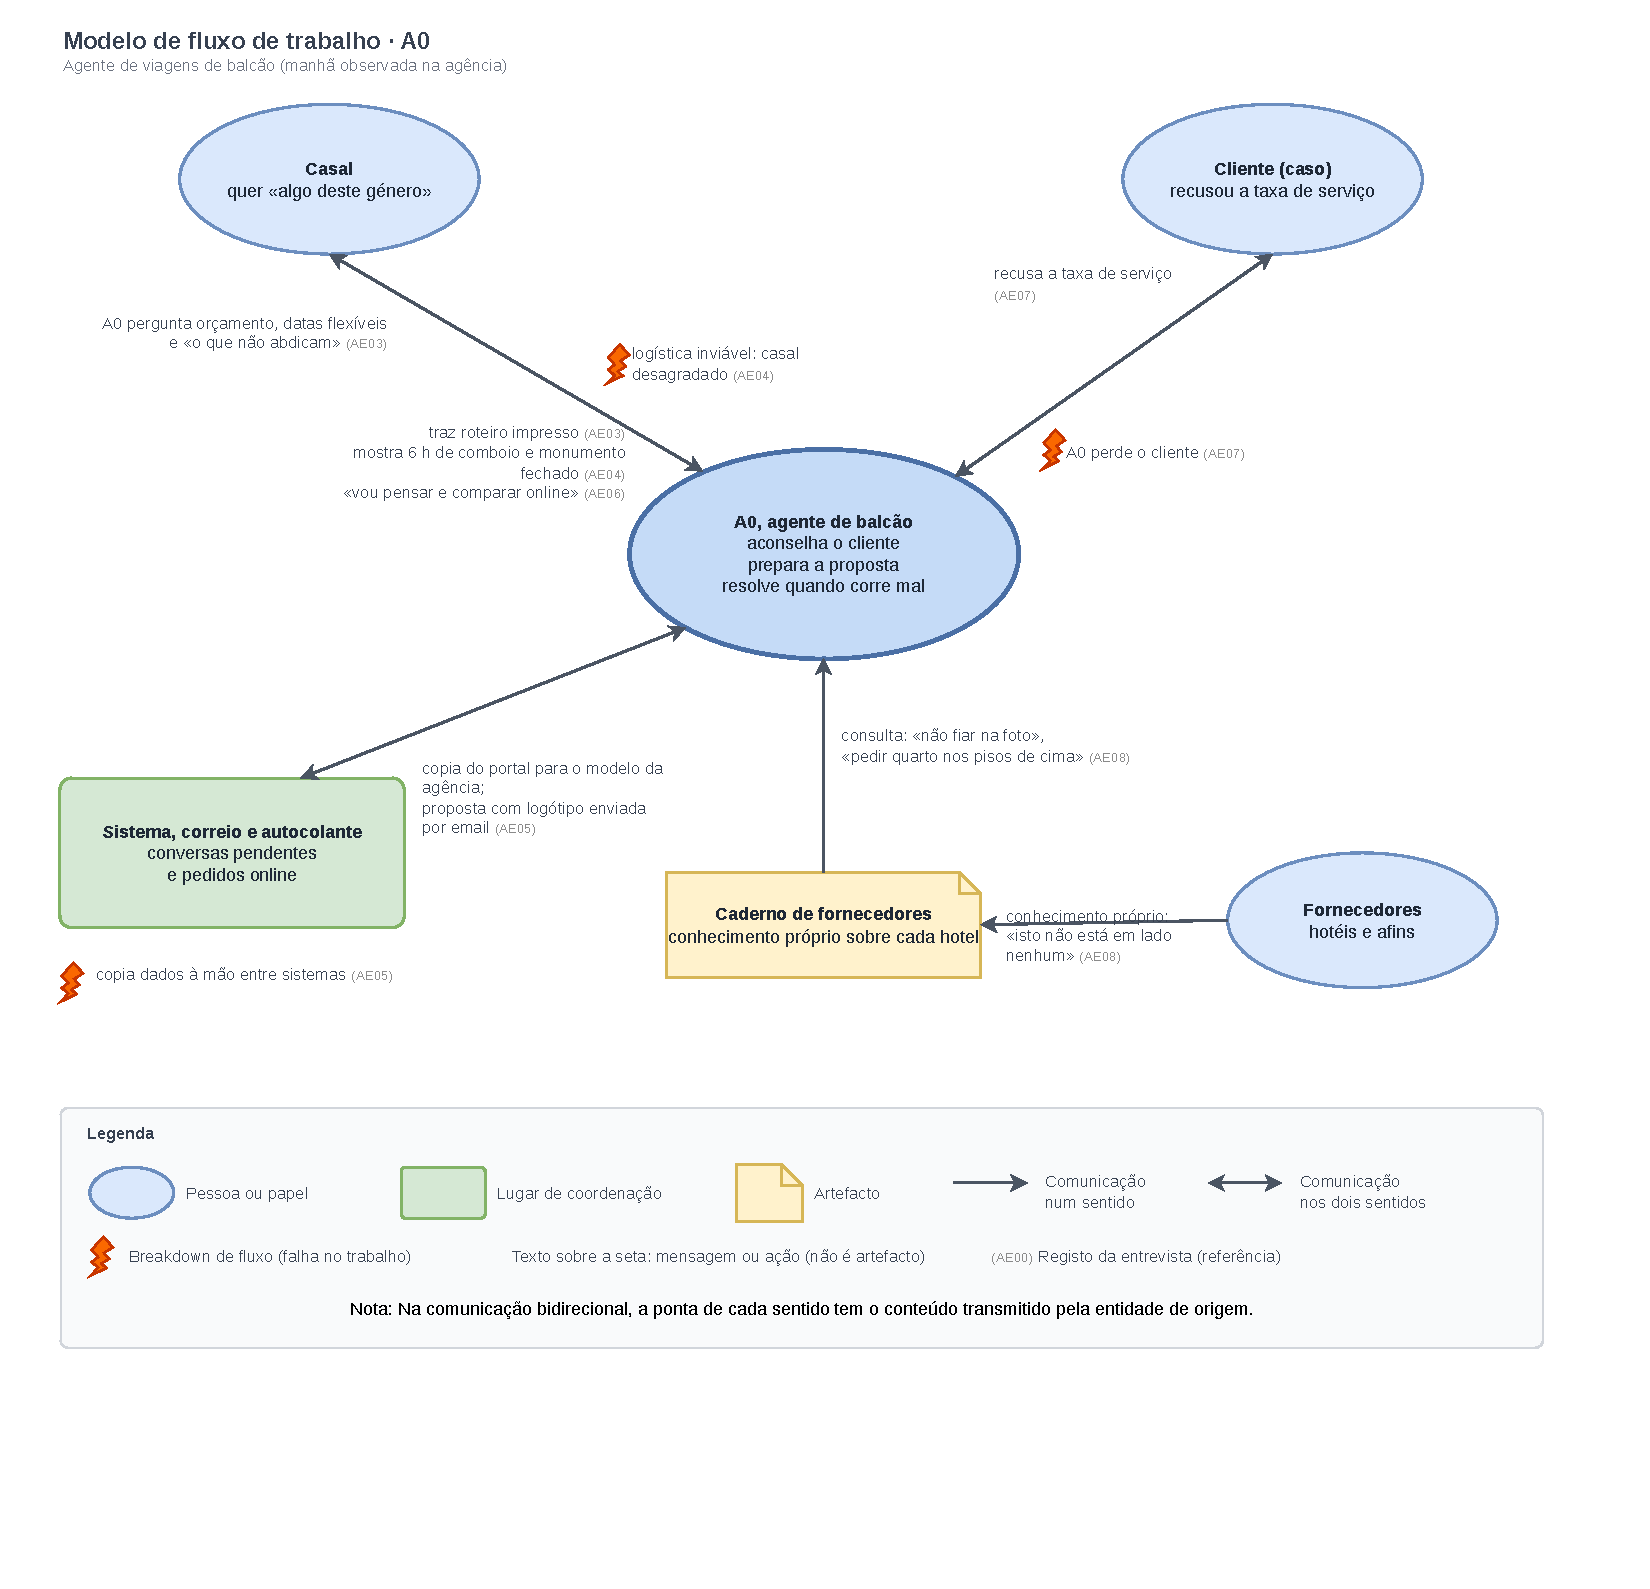
\includegraphics[width=\textwidth]{flow_models/individuais/A0flux.drawio.pdf}
\caption{Modelo de fluxo de A0 (agente de viagens de balcão).}
\label{fig:fluxo-a0}
\end{figure}

A0 está no centro de três frentes. \textbf{Com o cliente presencial} (o casal), 
A0 faz perguntas de descoberta («orçamento, datas flexíveis, o que não abdicam») 
e desfaz um roteiro inviável \reg{AE03, AE04}; o casal leva a proposta e diz que 
vai «pensar e comparar online» \reg{AE06}. \textbf{Com os sistemas da agência} 
(sistema de conversas pendentes, correio partilhado e um papel autocolante no ecrã), 
A0 recebe pedidos e copia à mão os dados do portal para o modelo de proposta da 
agência \reg{AE01, AE05}. \textbf{Com os fornecedores}, A0 recorre a um caderno 
pessoal com conhecimento que «não está em lado nenhum» \reg{AE08}.

\begin{table}[!htbp]
\centering\small
\begin{tabularx}{\textwidth}{@{}p{0.5cm}Lp{2.2cm}@{}}
\toprule
 & \textbf{Breakdown} & \textbf{Registo} \\
\midrule
\bolt & O roteiro do casal tem logística inviável; o casal fica desagradado. & AE04 \\
\bolt & Um cliente recusa a taxa de serviço porque «o site não cobra»; A0 perde-o. & AE07 \\
\bolt & A0 copia dados à mão entre sistemas para montar a proposta. & AE05 \\
\bottomrule
\end{tabularx}
\caption{\textit{Breakdowns} do modelo de fluxo de A0.}
\label{tab:bd-fluxo-a0}
\end{table}

\subsubsection{Fluxo de U0: viajante organizador(a)}

\begin{figure}[!htbp]
\centering
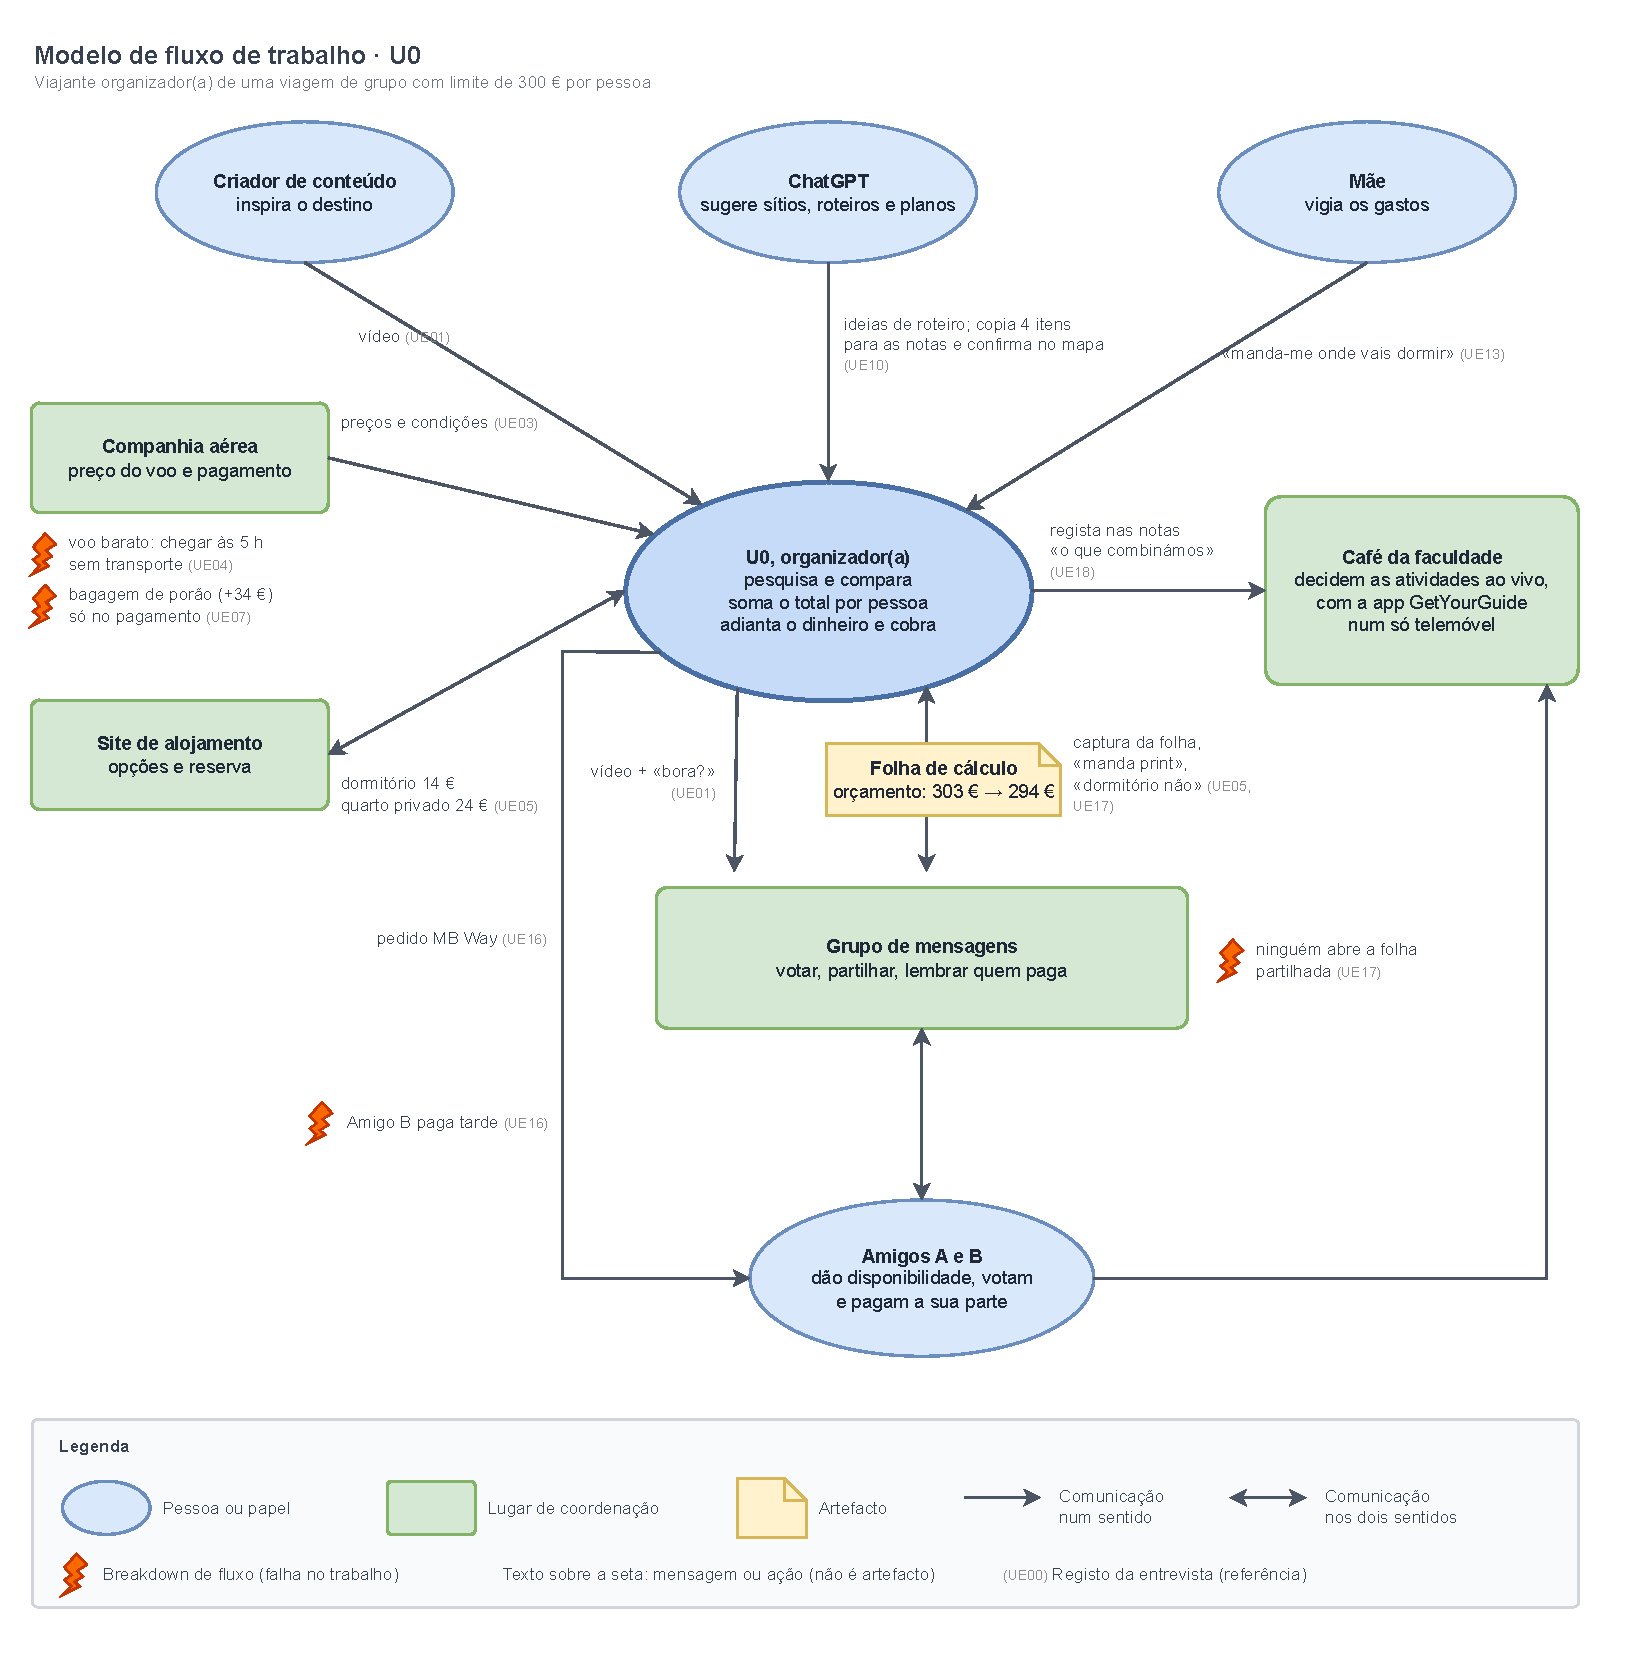
\includegraphics[width=\textwidth]{flow_models/individuais/FluxU0.drawio.pdf}
\caption{Modelo de fluxo de U0 (viajante que organiza uma viagem de grupo).}
\label{fig:fluxo-u0}
\end{figure}

U0 é o ponto por onde passa tudo. A viagem nasce de um vídeo de um 
criador de conteúdo \reg{UE01} e vai ganhando forma com ideias de 
roteiro pedidas ao ChatGPT e confirmadas no mapa \reg{UE10}. U0 
pesquisa sozinho(a) na companhia aérea e no site de alojamento \reg{UE03, UE05} 
e soma tudo numa folha de cálculo que vai de 303\,€ a 294\,€ \reg{UE06, UE12}. 
A coordenação com os amigos passa pelo grupo de mensagens, onde a folha só circula 
como captura de ecrã \reg{UE17}, e pelo café da faculdade, onde as atividades se 
decidem ao vivo num só telemóvel \reg{UE18}. U0 adianta o dinheiro e pede depois a 
parte de cada um \reg{UE16}. A mãe pede para saber onde U0 vai dormir \reg{UE13}.

\begin{table}[!htbp]
\centering\small
\begin{tabularx}{\textwidth}{@{}p{0.5cm}Lp{2.2cm}@{}}
\toprule
 & \textbf{Breakdown} & \textbf{Registo} \\
\midrule
\bolt & O voo barato obriga a chegar ao aeroporto às 5\,h, sem transporte. & UE04 \\
\bolt & A bagagem de porão (+34\,€) só aparece no pagamento. & UE07 \\
\bolt & Ninguém abre a folha partilhada; o grupo pede «print». & UE17 \\
\bolt & O Amigo~B paga tarde. & UE16 \\
\bottomrule
\end{tabularx}
\caption{\textit{Breakdowns} do modelo de fluxo de U0.}
\label{tab:bd-fluxo-u0}
\end{table}

%----------------------------------------------------------
\subsection{Modelos culturais}\label{sec:cultural}

O modelo cultural mostra as pressões, valores e expectativas que condicionam o 
trabalho~\cite{beyer1998}.

\subsubsection{Cultural de A0}

\begin{figure}[!htbp]
\centering
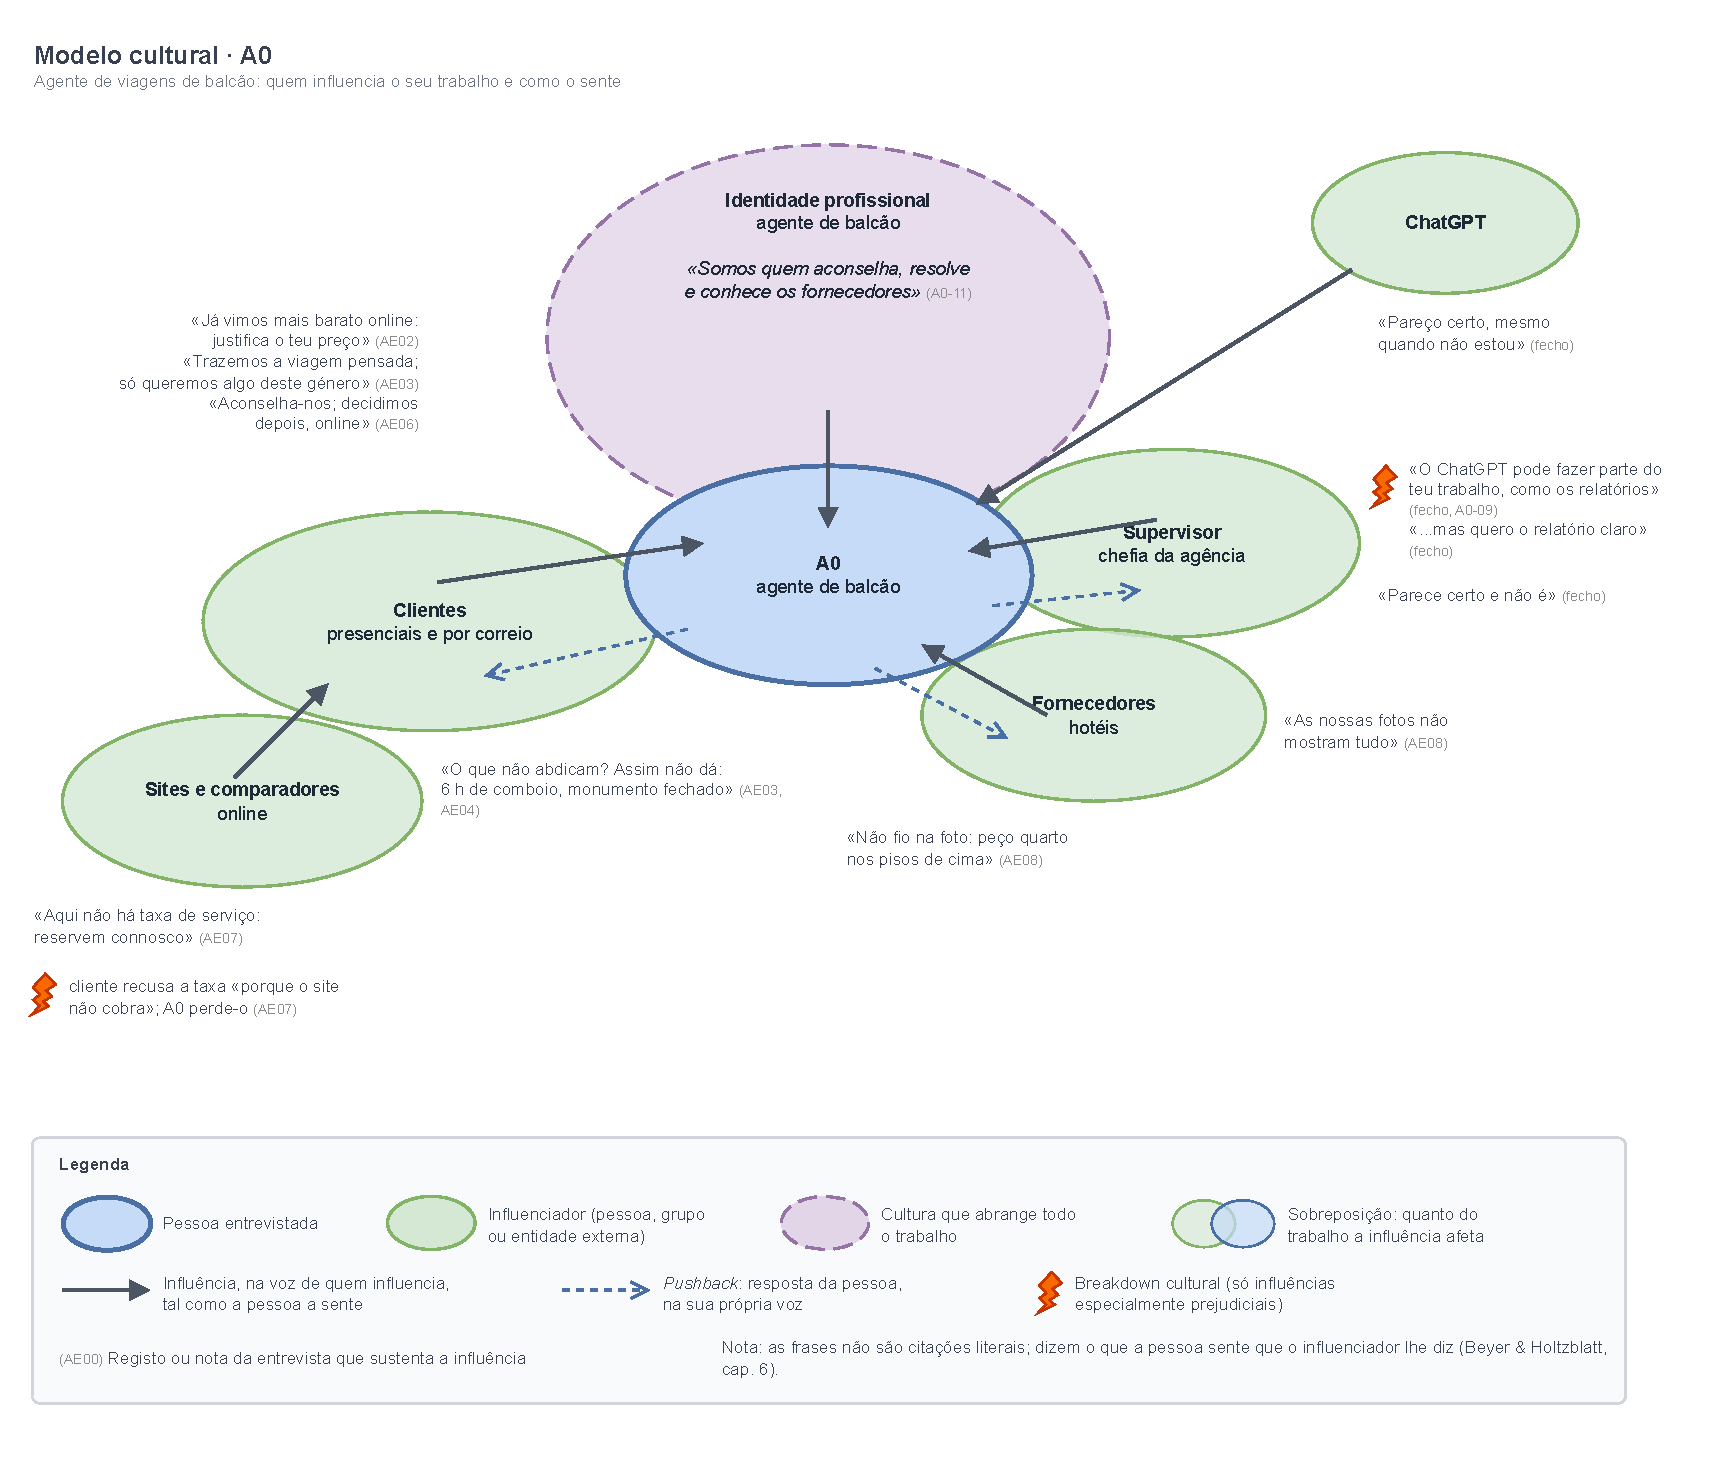
\includegraphics[width=\textwidth]{cultural_models/individuais/CulturalA0.drawio.pdf}
\caption{Modelo cultural de A0 (agente de viagens de balcão).}
\label{fig:cultural-a0}
\end{figure}

A identidade profissional pesa sobre todo o trabalho de A0: 
«somos quem aconselha, resolve e conhece os fornecedores» \reg{A0-11}. 
As influências mais fortes vêm dos \textbf{clientes}, que chegam com a 
viagem pensada e usam os preços online como pressão \reg{AE02, AE03, AE06}. 
Por trás deles estão os \textbf{sites e comparadores}, que não cobram taxa de serviço; 
essa influência chega a A0 através do cliente que recusa a taxa e se perde \reg{AE07}. 
O \textbf{supervisor} acha que o ChatGPT pode fazer parte do trabalho de A0, como 
redigir os relatórios, embora não goste quando o relatório sai confuso \reg{A0-09}, 
e o próprio \textbf{ChatGPT} é sentido como uma ferramenta que «parece certa, 
mesmo quando não está». A0 resiste: aponta ao cliente o que é inviável e diz ao 
supervisor que a IA «parece certa e não é».

\begin{table}[!htbp]
\centering\small
\begin{tabularx}{\textwidth}{@{}p{0.5cm}Lp{2.6cm}@{}}
\toprule
 & \textbf{Influência especialmente prejudicial} & \textbf{Registo} \\
\midrule
\bolt & Sites sem taxa de serviço levam o cliente a recusar a taxa; A0 perde o cliente. & AE07 \\
\bolt & O supervisor acha que o ChatGPT pode fazer parte do trabalho de A0 (os relatórios). & Fecho, A0-09 \\
\bottomrule
\end{tabularx}
\caption{\textit{Breakdowns} do modelo cultural de A0.}
\label{tab:bd-cult-a0}
\end{table}

\subsubsection{Cultural de U0}

\begin{figure}[!htbp]
\centering
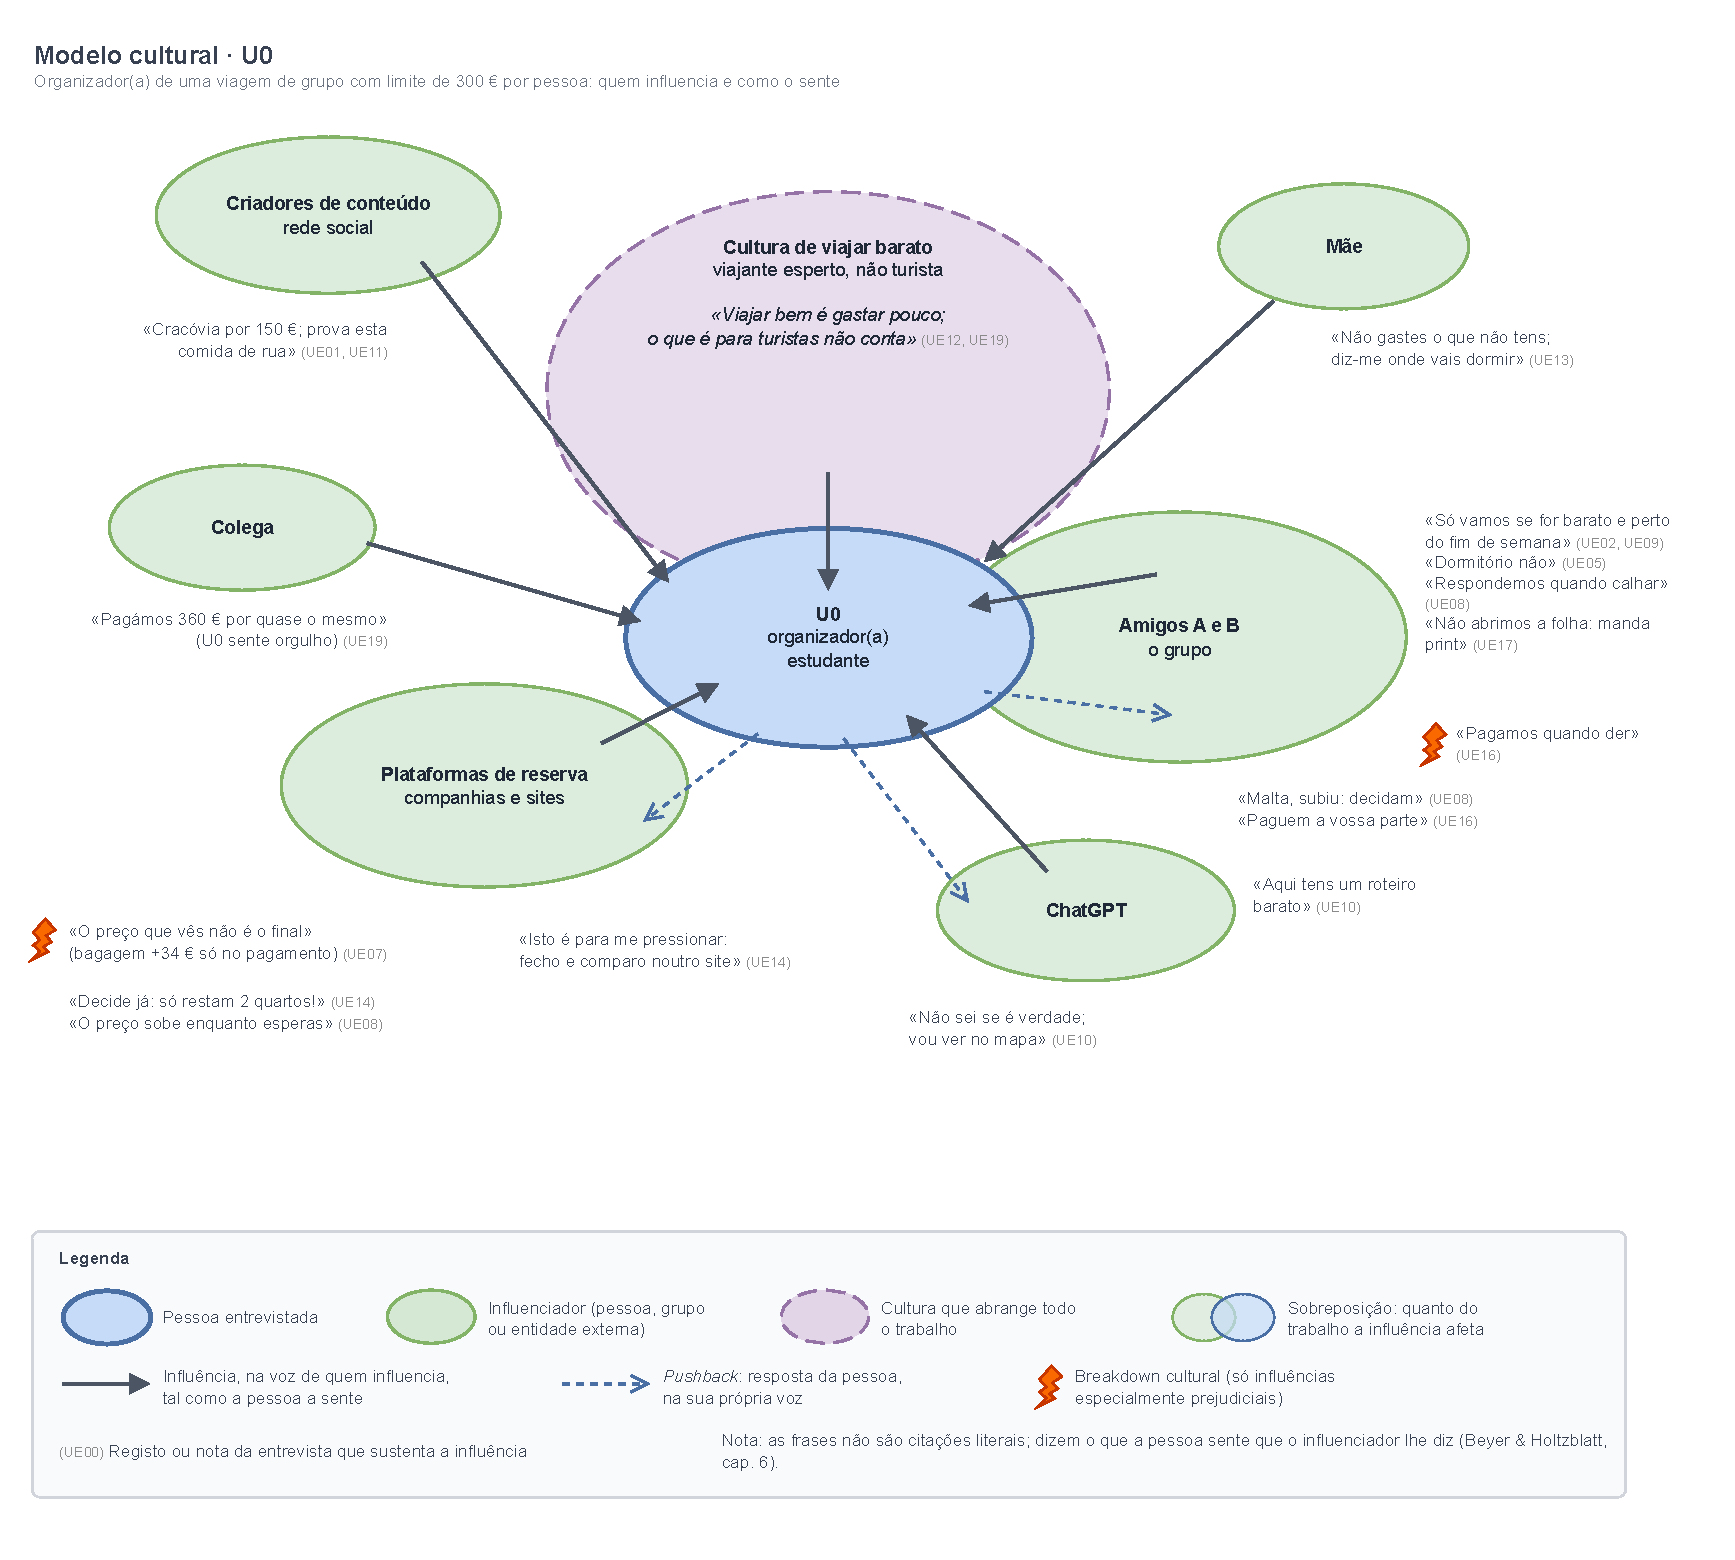
\includegraphics[width=\textwidth]{cultural_models/individuais/CulturalU0.drawio.pdf}
\caption{Modelo cultural de U0 (viajante organizador).}
\label{fig:cultural-u0}
\end{figure}

U0 vive dentro de uma \textbf{cultura de viajar barato}: «viajar bem é gastar pouco; 
o que é para turistas é armadilha». É ela que justifica cortar a mina de sal \reg{UE12} 
e que dá orgulho em pagar menos do que uma colega \reg{UE19}. Os \textbf{amigos} são 
a influência com mais peso: condicionam as datas e o tipo de alojamento, respondem 
devagar e pagam tarde \reg{UE02, UE05, UE08, UE16, UE17}. As 
\textbf{plataformas de reserva} são sentidas como adversárias: 
escondem custos e pressionam com «só restam 2 quartos!» \reg{UE07, UE14}. 
U0 resiste: fecha o separador e compara noutro site, pede ao grupo que 
decida e pague, e verifica no mapa o que o ChatGPT sugere \reg{UE08, UE10, UE14, UE16}. 
A \textbf{mãe} e os \textbf{criadores de conteúdo} têm influências mais 
pontuais \reg{UE01, UE11, UE13}.

\begin{table}[!htbp]
\centering\small
\begin{tabularx}{\textwidth}{@{}p{0.5cm}Lp{2.6cm}@{}}
\toprule
 & \textbf{Influência especialmente prejudicial} & \textbf{Registo} \\
\midrule
\bolt & As plataformas mostram um preço que não é o final (bagagem só no pagamento). & UE07 \\
\bolt & O grupo paga «quando der»: U0 fica a fazer de banco. & UE16 \\
\bottomrule
\end{tabularx}
\caption{\textit{Breakdowns} do modelo cultural de U0.}
\label{tab:bd-cult-u0}
\end{table}

%----------------------------------------------------------
\subsection{Modelos de sequência}\label{sec:sequencia}

%----------------------------------------------------------
\subsection{Modelos de artefacto}\label{sec:artefacto}

%----------------------------------------------------------
\subsection{Modelos físicos}\label{sec:fisico}

%==========================================================
\section{Consolidação dos modelos}\label{sec:consolidacao}

A consolidação junta os modelos individuais para mostrar a estrutura comum do trabalho, em vez de casos isolados~\cite[cap.~9]{beyer1998}. Foi aplicada às duas sessões (A0 e U0), que representam as duas populações do problema: quem planeia a viagem e quem a planeia profissionalmente.

%----------------------------------------------------------
\subsection{Fluxo consolidado}\label{sec:fluxo-cons}

\paragraph{Método.} Seguiram-se os passos do livro~\cite[pp.~163--170]{beyer1998}:
\begin{enumerate}
  \item listar as responsabilidades de cada pessoa, grupo e lugar nos fluxos individuais;
  \item agrupar as responsabilidades em \textbf{papéis}, cada um com uma intenção principal; só é papel o que se poderia atribuir a uma pessoa contratada para isso;
  \item juntar papéis semelhantes vindos de modelos diferentes e dar-lhes um nome simples;
  \item redesenhar as comunicações e os artefactos entre papéis, com nomes abstratos;
  \item copiar os \textit{breakdowns} dos modelos individuais;
  \item colorir cada papel pela população que o desempenha (viajante, agente ou não entrevistado).
\end{enumerate}

\begin{figure}[!htbp]
\centering
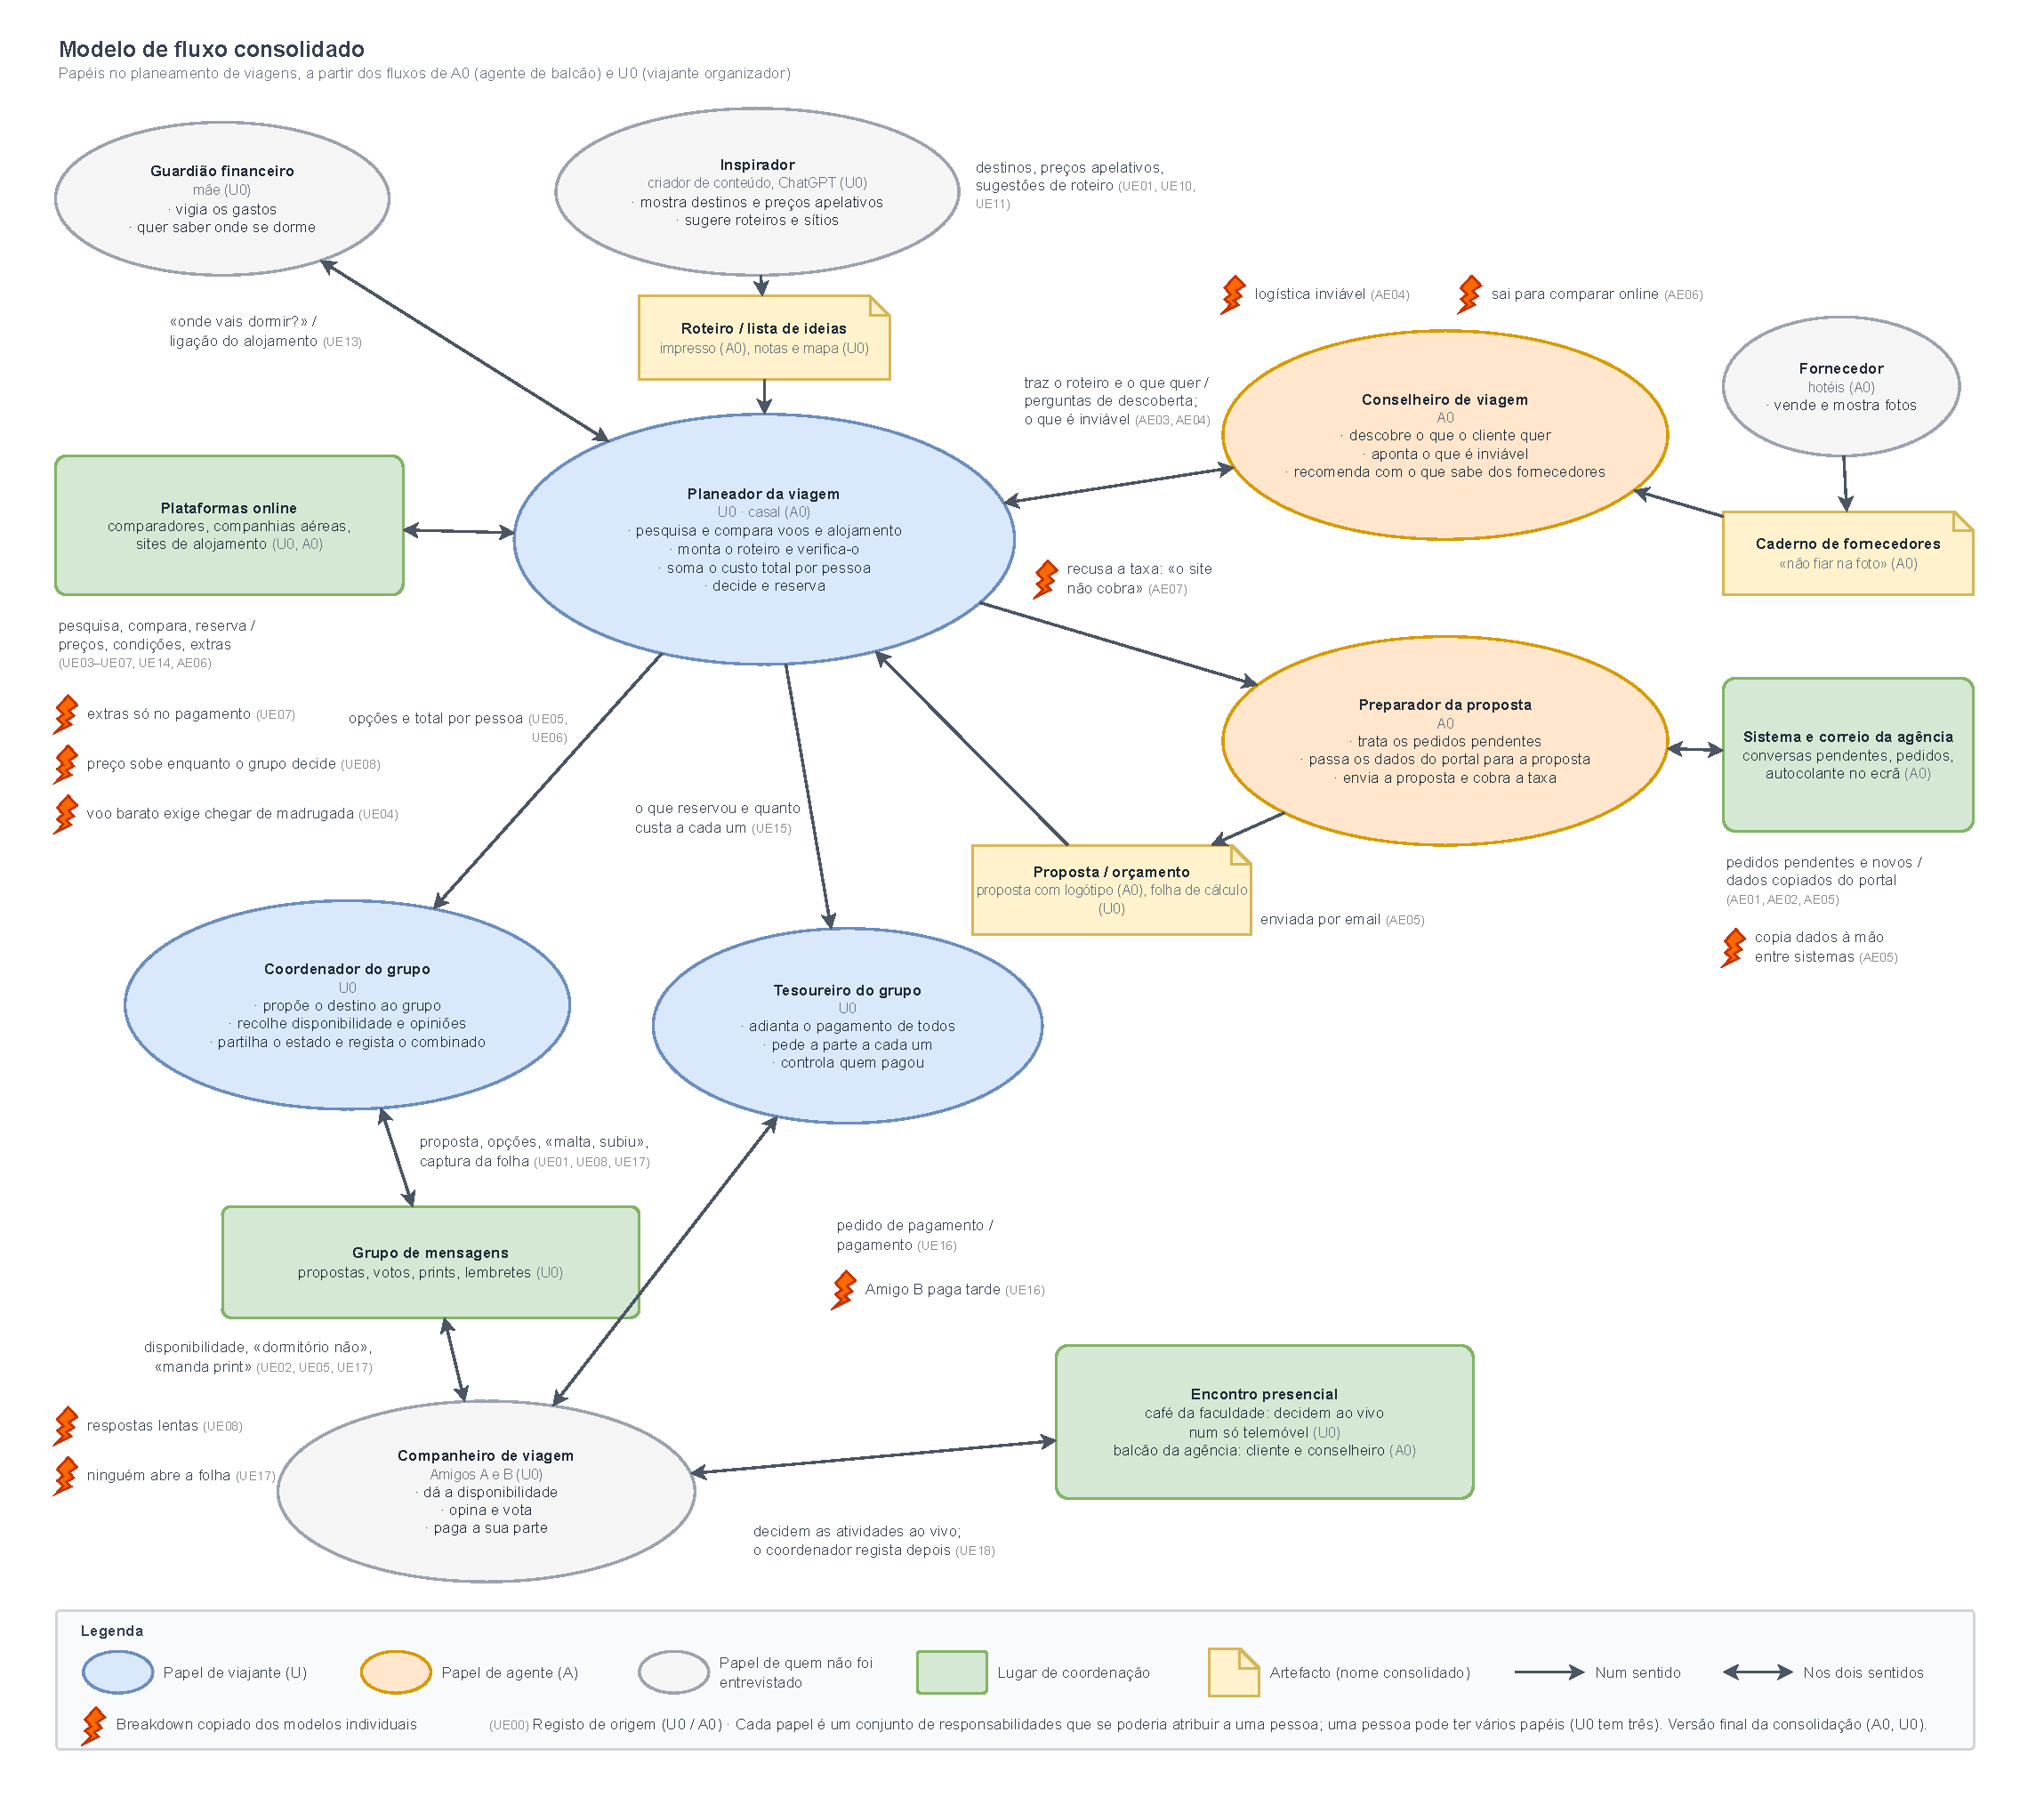
\includegraphics[width=\textwidth]{flow_models/consolidado/FluxoConsolidado.drawio.pdf}
\caption{Modelo de fluxo consolidado (A0 e U0).}
\label{fig:fluxo-cons}
\end{figure}

\paragraph{Papéis.} A Tabela~\ref{tab:papeis-cons} mostra os nove papéis identificados e quem os desempenha.

\begin{table}[!htbp]
\centering\small
\begin{tabularx}{\textwidth}{@{}p{3.4cm}Lp{2.8cm}@{}}
\toprule
\textbf{Papel} & \textbf{Responsabilidades} & \textbf{Desempenhado por} \\
\midrule
\rowcolor{blue!6} Planeador da viagem & Pesquisa e compara voos e alojamento; monta o roteiro e verifica-o; soma o custo total por pessoa; decide e reserva. & U0; casal (A0) \\
\rowcolor{blue!6} Coordenador do grupo & Propõe o destino; recolhe disponibilidade e opiniões; partilha o estado e regista o combinado. & U0 \\
\rowcolor{blue!6} Tesoureiro do grupo & Adianta o pagamento de todos; pede a parte a cada um; controla quem pagou. & U0 \\
\rowcolor{orange!10} Conselheiro de viagem & Descobre o que o cliente quer; aponta o que é inviável; recomenda com o que sabe dos fornecedores. & A0 \\
\rowcolor{orange!10} Preparador da proposta & Trata os pedidos pendentes; passa os dados do portal para a proposta; envia-a e cobra a taxa. & A0 \\
Inspirador & Mostra destinos e preços apelativos; sugere roteiros e sítios. & Criador de conteúdo, ChatGPT \\
Guardião financeiro & Vigia os gastos; quer saber onde se dorme. & Mãe de U0 \\
Companheiro de viagem & Dá a disponibilidade; opina e vota; paga a sua parte. & Amigos A e B \\
Fornecedor & Vende e mostra fotos. & Hotéis \\
\bottomrule
\end{tabularx}
\caption{Papéis do fluxo consolidado. Azul: viajante; laranja: agente; branco: não entrevistado.}
\label{tab:papeis-cons}
\end{table}

\paragraph{Lugares e artefactos consolidados.} \textbf{Plataformas online} junta comparadores, companhias aéreas e sites de alojamento (U0, A0). \textbf{Encontro presencial} junta o café da faculdade (U0) e o balcão da agência (A0). \textbf{Roteiro / lista de ideias} junta o roteiro impresso do casal (A0) com as notas e a lista no mapa de U0. \textbf{Proposta / orçamento} junta a proposta com logótipo (A0) com a folha de cálculo de U0.

\paragraph{O que o fluxo consolidado mostra.}
\begin{itemize}
  \item \textbf{Uma só pessoa acumula três papéis.} U0 é planeador, coordenador e tesoureiro. Não há nenhuma ferramenta que apoie os três ao mesmo tempo; cada papel tem o seu sítio (folha, grupo de mensagens, pedido de pagamento).
  \item \textbf{O agente desempenha papéis que o viajante faz sozinho.} O conselheiro (descobrir o que se quer, apontar o que é inviável) faz o que U0 faz ao verificar no mapa as sugestões da IA. É este o espaço que o \projeto{} quer ocupar.
  \item \textbf{A proposta é o artefacto central nos dois mundos.} Para o agente é o documento com logótipo; para o viajante é a folha de cálculo. Nos dois casos é montada à mão a partir de dados copiados de outros sistemas.
  \item \textbf{Os \textit{breakdowns} concentram-se nas passagens entre papéis}: entre plataformas e planeador (custos escondidos, preços que sobem), entre coordenador e companheiros (respostas lentas, folha que ninguém abre) e entre tesoureiro e companheiros (pagamentos em atraso).
\end{itemize}

%----------------------------------------------------------
\subsection{Cultural consolidado}\label{sec:cultural-cons}

\paragraph{Método.} Seguiram-se os passos do livro~\cite[pp.~190--198]{beyer1998}:
\begin{enumerate}
  \item catalogar os influenciadores dos modelos individuais;
  \item agrupar os que condicionam o trabalho da mesma forma;
  \item recolher as influências e agrupá-las pelo par de influenciadores entre os quais vão;
  \item eliminar duplicados e escolher uma redação que mostre o tom emocional da influência;
  \item desenhar o modelo final e copiar os \textit{breakdowns}.
\end{enumerate}

\begin{figure}[!htbp]
\centering
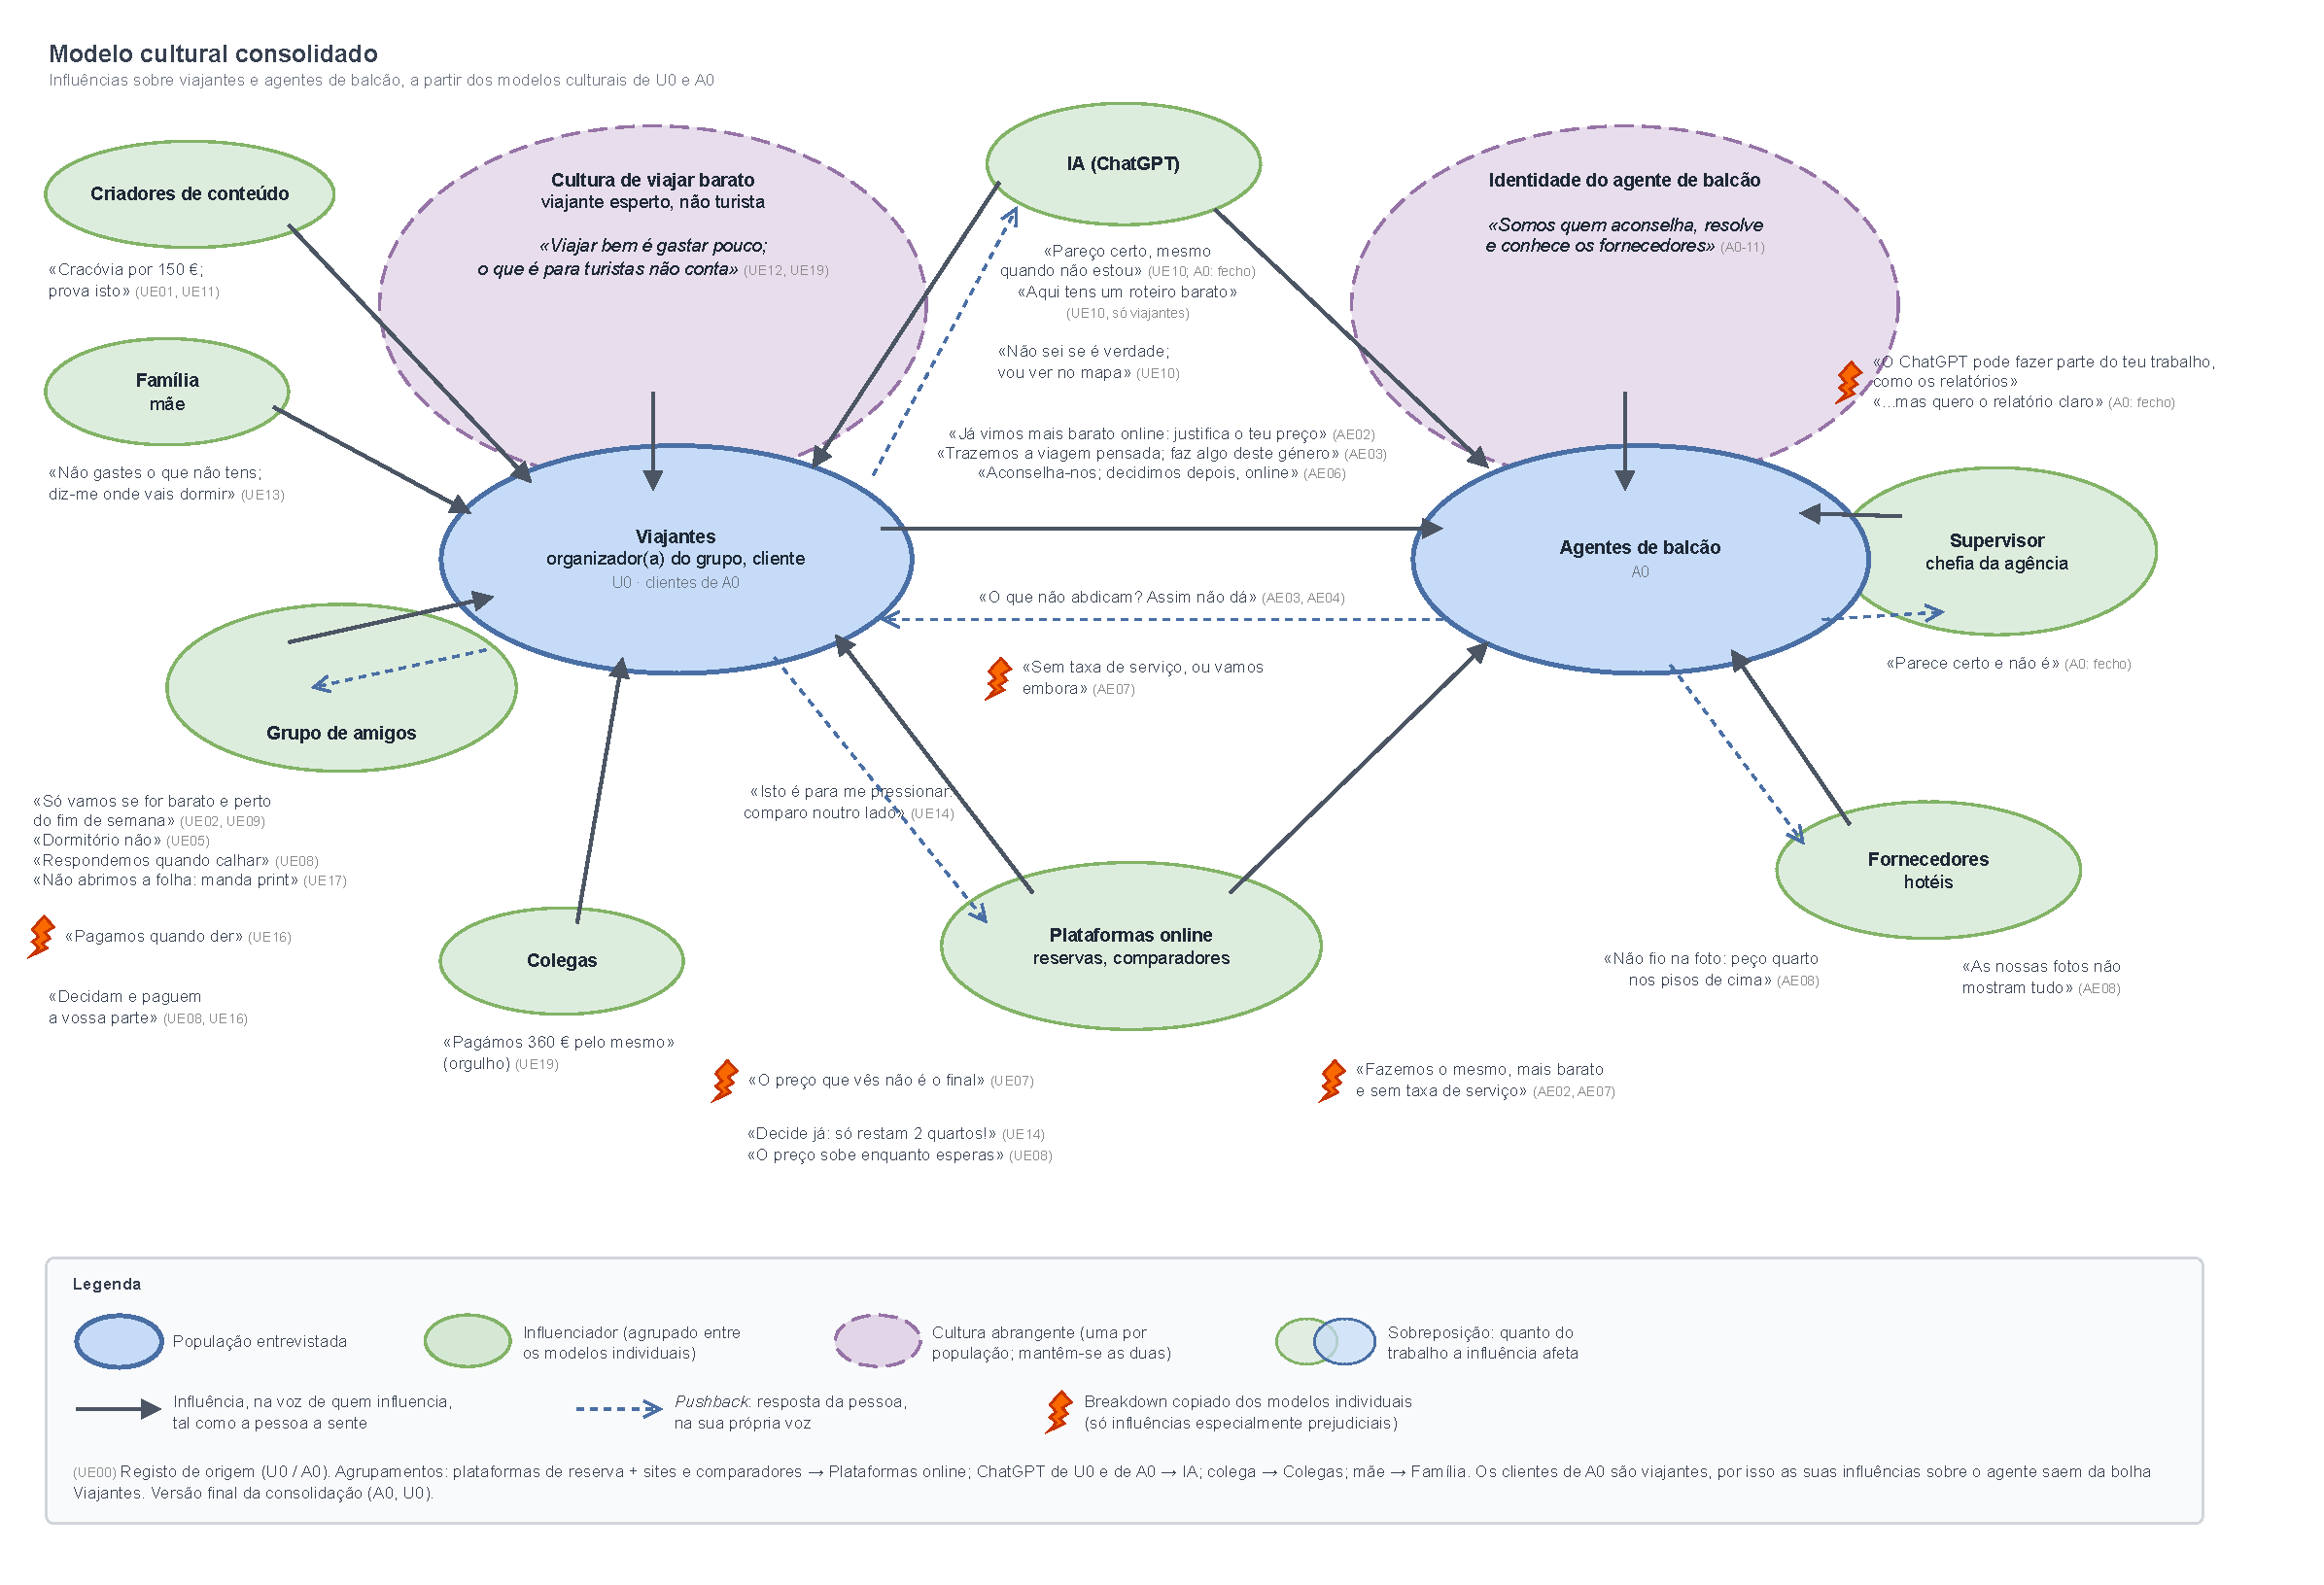
\includegraphics[width=\textwidth]{cultural_models/consolidado/CulturalConsolidado.drawio.pdf}
\caption{Modelo cultural consolidado (A0 e U0).}
\label{fig:cultural-cons}
\end{figure}

\begin{table}[!htbp]
\centering\small
\begin{tabularx}{\textwidth}{@{}p{4.4cm}p{3.4cm}L@{}}
\toprule
\textbf{Nos modelos individuais} & \textbf{No modelo consolidado} & \textbf{Porquê} \\
\midrule
Plataformas de reserva (U0); sites e comparadores (A0) & Plataformas online & Pressionam da mesma forma: preço, urgência, ausência de taxa. \\
ChatGPT (U0); ChatGPT (A0) & IA (ChatGPT) & A mesma ferramenta, sentida com a mesma desconfiança. \\
Clientes (A0) & Viajantes & Os clientes de A0 são viajantes; as suas influências saem da bolha Viajantes. \\
Colega (U0) & Colegas & Referência de preço entre pares. \\
Mãe (U0) & Família & Financia e vigia. \\
Amigos A e B (U0) & Grupo de amigos & -- \\
Supervisor, fornecedores (A0) & Supervisor, fornecedores & -- \\
\bottomrule
\end{tabularx}
\caption{Agrupamento dos influenciadores na consolidação cultural.}
\label{tab:agrup-cult}
\end{table}

\paragraph{O que o cultural consolidado mostra.}
\begin{itemize}
  \item \textbf{Duas culturas diferentes, mantidas lado a lado.} Os viajantes vivem na cultura de viajar barato; os agentes na identidade de quem aconselha e conhece os fornecedores. O livro recomenda manter culturas diferentes quando a consolidação as revela.
  \item \textbf{As duas populações influenciam-se.} Os viajantes pressionam o agente com os preços online e recusam a taxa; o agente responde apontando o que é inviável.
  \item \textbf{As plataformas online pesam sobre as duas populações}: sobre o viajante como adversárias (custos escondidos, falsa escassez) e sobre o agente como concorrentes («fazemos o mesmo, sem taxa»).
  \item \textbf{A desconfiança da IA é comum.} «Pareço certo, mesmo quando não estou» aparece nos dois modelos: o viajante verifica no mapa, o agente teme ser substituído por algo que erra.
\end{itemize}

%----------------------------------------------------------
\subsection{Restantes modelos consolidados}\label{sec:outros-cons}

\pendente{Gonçalo (sequência e artefacto) e Zé Pedro (físico)}{%
O enunciado pede pelo menos o fluxo, a sequência e mais um modelo consolidado. Incluir aqui a sequência consolidada (obrigatória) e, se houver, o artefacto e o físico consolidados, com o mesmo formato: método, figura e o que o modelo mostra.}

%----------------------------------------------------------
\subsection{Implicações para o design}\label{sec:implicacoes}

A Tabela~\ref{tab:implicacoes} liga os principais \textit{breakdowns} dos modelos de fluxo e culturais às hipóteses de produto do \textit{backlog} da equipa (Apêndice~\ref{anx:hipoteses}). Esta ligação garante que cada hipótese assenta em dados de campo e não em suposições.

\begin{table}[!htbp]
\centering\small
\begin{tabularx}{\textwidth}{@{}Lp{2.1cm}Lp{1.6cm}@{}}
\toprule
\textbf{Breakdown ou influência} & \textbf{Origem} & \textbf{Implicação para o design} & \textbf{Hipótese} \\
\midrule
Bagagem e extras só aparecem no pagamento & UE07 & Mostrar o custo total real por pessoa antes de qualquer reserva. & US-02, RF-03 \\
Voo barato exige chegar de madrugada sem transporte & UE04 & Incluir custo e tempo de chegada ao aeroporto nas comparações. & US-03, RF-04 \\
Preço sobe enquanto o grupo decide; respostas lentas & UE08 & Avisar de variações de preço e dar um prazo de decisão ao grupo. & US-05, RF-06 \\
Ninguém abre a folha; «manda print» & UE17 & Partilhar a proposta num link legível sem conta, com votação. & US-04, RF-05 \\
Organizador adianta o dinheiro; amigo paga tarde & UE15, UE16 & Dividir despesas e acompanhar quem já pagou. & US-06, RF-07 \\
«Só restam 2 quartos!» sentido como manipulação & UE14 & Não usar urgência nem escassez falsas. & RNF-02 \\
IA «parece certa e não é» & UE10; fecho A0 & Explicar porque recomenda e de onde vêm os preços. & US-09, RF-10 \\
Roteiro do cliente com logística inviável & AE04 & Validar a logística (distâncias, horários) antes de propor. & RF-02 \\
Supervisor vê a IA como substituto do agente & Fecho A0 & Permitir revisão humana da proposta por um agente. & US-13, RF-13 \\
Agente copia dados à mão entre sistemas & AE05 & Gerar a proposta diretamente a partir das opções escolhidas. & RF-02 \\
\bottomrule
\end{tabularx}
\caption{Dos \textit{breakdowns} às hipóteses de produto.}
\label{tab:implicacoes}
\end{table}

%==========================================================
\section{Personas}\label{sec:personas}

As personas foram construídas a partir das duas entrevistas contextuais e dos modelos que delas resultaram, e não a partir do que a equipa acha que os utilizadores fazem. Há uma persona para cada lado do problema: a \textbf{organizadora do grupo}, construída a partir de U0, e o \textbf{agente de balcão}, construído a partir de A0. Cada campo remete para os registos que o sustentam. O que não foi observado nem contado está marcado como \textit{suposição}.

Os nomes e as fotografias são fictícios, para proteger o anonimato dos participantes.

%----------------------------------------------------------
% Caixa de persona: \begin{persona}{Nome}{Arquétipo} ... \end{persona}
\newtcolorbox{persona}[2]{colback=roamly!4,colframe=roamly,arc=2pt,boxrule=0.8pt,
  fonttitle=\bfseries,title={#1 \hfill\normalfont\small #2},breakable=false}
\newcommand{\campo}[1]{\textbf{#1}}
\newcommand{\suposicao}{\textit{\textcolor{pendente}{(suposição)}}}

%----------------------------------------------------------
\subsection{Inês: a organizadora do grupo}\label{sec:persona-ines}

\begin{persona}{Inês Carvalho, 20 anos}{Arquétipo: organizadora do grupo · caçadora de promoções}
\begin{minipage}[t]{0.26\textwidth}
\vspace{0pt}

\includegraphics[width=\linewidth]{figuras/ines.png}\\[2pt]
{\footnotesize Imagem gerada por IA;}
\end{minipage}\hfill
\begin{minipage}[t]{0.7\textwidth}
\vspace{0pt}\small
\begin{tabularx}{\textwidth}{@{}p{2.6cm}L@{}}
\campo{Ocupação} & Estudante do 2.º ano de licenciatura \reg{perfil U0} \\
\campo{Local} & Cidade sem aeroporto;\reg{perfil U0, UE03} \\
\campo{Dinheiro} & Mesada ($\approx$250\,€) e explicações ($\approx$120\,€); $\approx$380\,€ poupados para viajar; cartão de débito e MB Way, sem crédito \reg{perfil U0} \\
\campo{Literacia digital} & Alta. Usa comparadores com datas flexíveis, reaproveita folhas de cálculo, pede roteiros ao ChatGPT e usa MB Way e GetYourGuide \reg{UE03, UE06, UE10, UE16, UE18} \\
\campo{Dispositivos} & Telemóvel e portátil \reg{UE01, UE06} \\
\end{tabularx}
\end{minipage}

\medskip
\begin{tcolorbox}[colback=white,colframe=roamly!40,boxrule=0.4pt,arc=1pt,left=6pt,right=6pt,top=3pt,bottom=3pt]
\small\itshape «Os sites estão sempre a tentar enganar-me. A viagem barata é a que eu monto e verifico peça a peça, e sou eu que ponho o grupo a andar.»
\end{tcolorbox}
\end{persona}

\begin{table}[H]
\centering\small
\begin{tabularx}{\textwidth}{@{}p{3.2cm}L@{}}
\toprule
\textbf{Objetivos com o Roamly} &
\begin{itemize}[topsep=0pt]
  \item Ver o \textbf{custo real por pessoa}, com extras e deslocação ao aeroporto, antes de decidir \reg{UE04, UE07}.
  \item Partir do \textbf{orçamento e das datas}, não do destino \reg{UE03}.
  \item Pôr o grupo a decidir \textbf{antes de o preço subir} \reg{UE08}.
  \item Saber quem já pagou sem ter de andar a cobrar \reg{UE16}.
\end{itemize} \\
\midrule
\textbf{Motivações} &
\begin{itemize}[topsep=0pt]
  \item Viajar é o que mais gosta de fazer, e poupa para isso \reg{conversa U0}.
  \item Orgulho em gastar menos do que os outros \reg{UE19}.
  \item Não ser manipulada por quem vende \reg{UE14}.
  \item Que os amigos fiquem contentes: as escolhas são de preço, «mas sempre a pensar nos amigos» \reg{fecho U0}.
\end{itemize} \\
\midrule
\textbf{Como mede o sucesso} &
\begin{itemize}[topsep=0pt]
  \item O total fica dentro dos 300\,€ por pessoa, tudo incluído \reg{perfil U0}.
  \item Pagou menos do que outros pela mesma viagem (294\,€ contra os 360\,€ de uma colega) \reg{UE19}.
  \item Nenhuma surpresa no momento de pagar \reg{UE07}.
\end{itemize} \\
\midrule
\textbf{Atritos atuais} &
\begin{itemize}[topsep=0pt]
  \item Copia à mão os preços de cada site para uma folha de cálculo; o total muda três vezes (303\,€, 322\,€, 294\,€) \reg{UE06, UE09, UE12}.
  \item A bagagem (+34\,€) só aparece no pagamento \reg{UE07}.
  \item O voo mais barato obriga a chegar ao aeroporto de madrugada, sem transporte \reg{UE04}.
  \item O grupo demora dois dias a responder e o voo sobe 19\,€ \reg{UE08}.
  \item Ninguém abre a folha partilhada: «manda print» \reg{UE17}.
  \item Tem de verificar no mapa tudo o que o ChatGPT sugere \reg{UE10}.
\end{itemize} \\
\midrule
\textbf{Ansiedades e \textit{dealbreakers}} &
\begin{itemize}[topsep=0pt]
  \item Adiantar o dinheiro de todos e esperar até ao fim do mês para o reaver \reg{UE15, UE16, fecho U0}.
  \item «Não gastes o que não tens»: a pressão da família sobre os gastos \reg{UE13}.
  \item \textbf{\textit{Dealbreaker}:} pressão de compra. Perante «só restam 2 quartos!», fecha o separador e vai a outro site \reg{UE14}.
  \item \textbf{\textit{Dealbreaker}:} preços ou sugestões sem origem que possa confirmar \reg{UE10, fecho U0}.
  \item \textbf{\textit{Dealbreaker}:} pagar pelo serviço, quando poupar é o objetivo \suposicao.
\end{itemize} \\
\bottomrule
\end{tabularx}
\caption{Persona Inês: objetivos, motivações, atritos e ansiedades.}
\label{tab:persona-ines}
\end{table}

%----------------------------------------------------------
\subsection{Rui: o agente de balcão}\label{sec:persona-rui}

\begin{persona}{Rui Mendes}{Arquétipo: agente de viagens de balcão · conselheiro}
\begin{minipage}[t]{0.26\textwidth}
\vspace{0pt}

\includegraphics[width=\linewidth]{figuras/rui.png}\\[2pt]
{\footnotesize Imagem gerada por IA;}
\end{minipage}\hfill
\begin{minipage}[t]{0.7\textwidth}
\vspace{0pt}\small
\begin{tabularx}{\textwidth}{@{}p{2.6cm}L@{}}
\campo{Ocupação} & Agente de viagens de balcão há 12 anos, na mesma agência \reg{perfil A0} \\
\campo{Local} & Agência de rua, atrás do balcão; os clientes vêm até ele \reg{AE03} \\
\campo{Idade} & Cerca de 40 anos \suposicao \\
\campo{Literacia digital} & Média. Trabalha todos os dias com várias aplicações em paralelo (sistema de conversas, correio partilhado, portal, modelo da agência), mas guarda o que mais importa em papel: autocolante no monitor e caderno de fornecedores \reg{AE01, AE05, AE08} \\
\campo{Responde a} & Um supervisor que espera que o ChatGPT faça parte do trabalho \reg{fecho A0} \\
\end{tabularx}
\end{minipage}

\medskip
\begin{tcolorbox}[colback=white,colframe=roamly!40,boxrule=0.4pt,arc=1pt,left=6pt,right=6pt,top=3pt,bottom=3pt]
\small\itshape «O meu valor está no que eu sei e os sites não mostram. Mas o cliente só vê a taxa e vai comparar online.»
\end{tcolorbox}
\end{persona}

\begin{table}[H]
\centering\small
\begin{tabularx}{\textwidth}{@{}p{3.2cm}L@{}}
\toprule
\textbf{Objetivos com o Roamly} &
\begin{itemize}[topsep=0pt]
  \item Montar a proposta \textbf{sem copiar dados à mão} entre sistemas \reg{AE05, fecho A0}.
  \item Mostrar ao cliente \textbf{o que vale a taxa} de serviço \reg{AE07}.
  \item Ter à mão, ao preparar a proposta, o que sabe sobre cada fornecedor \reg{AE08}.
  \item Rever e assinar tudo antes de enviar \suposicao{} \reg{A0-14}.
\end{itemize} \\
\midrule
\textbf{Motivações} &
\begin{itemize}[topsep=0pt]
  \item Ser quem aconselha, se responsabiliza e resolve quando corre mal \reg{fecho A0}.
  \item Ser reconhecido por conhecer os fornecedores \reg{fecho A0, AE08}.
  \item Poupar tempo: a preparação ocupa «grande parte da manhã» \reg{fecho A0}.
  \item Não perder clientes para a concorrência online \reg{AE06, AE07}.
\end{itemize} \\
\midrule
\textbf{Como mede o sucesso} &
\begin{itemize}[topsep=0pt]
  \item A proposta sai «o mais rápido possível» \reg{AE05}.
  \item O cliente aceita a proposta e paga a taxa, em vez de ir «pensar e comparar online» \reg{AE06, AE07}.
  \item A viagem corre bem, ou ele resolve o que corre mal \reg{fecho A0}.
\end{itemize} \\
\midrule
\textbf{Atritos atuais} &
\begin{itemize}[topsep=0pt]
  \item Copia à mão os dados do portal para o modelo da agência \reg{AE05}.
  \item Trabalha com várias aplicações ao mesmo tempo e lembretes em papel \reg{AE01}.
  \item Os clientes trazem roteiros inviáveis (cidades a 6\,h de comboio, monumento fechado); ao desfazê-los, passa por «desmancha-prazeres» \reg{AE04, conversa A0}.
  \item Os clientes usam preços online como pressão: «menos 10 ou 20 euros por noite» \reg{AE02}.
  \item O que sabe sobre fornecedores só está no seu caderno \reg{AE08}.
\end{itemize} \\
\midrule
\textbf{Ansiedades e \textit{dealbreakers}} &
\begin{itemize}[topsep=0pt]
  \item Que os clientes deixem de precisar da agência \reg{conversa A0}.
  \item Que o supervisor ache que o ChatGPT o substitui \reg{fecho A0}.
  \item \textbf{\textit{Dealbreaker}:} uma IA que «parece certa e não é», porque o erro cai sobre ele \reg{fecho A0}.
  \item \textbf{\textit{Dealbreaker}:} uma ferramenta que o reduza a intermediário \reg{A0-11}.
\end{itemize} \\
\bottomrule
\end{tabularx}
\caption{Persona Rui: objetivos, motivações, atritos e ansiedades.}
\label{tab:persona-rui}
\end{table}


%==========================================================
\section{Diagrama de afinidade}\label{sec:afinidade}

O diagrama de afinidade organiza as notas de interpretação das duas sessões (A0-01 a A0-15 e U0-01 a U0-21) por semelhança de significado, de baixo para cima, para revelar os temas comuns a toda a população~\cite[cap.~9]{beyer1998}. As notas agrupam-se em grupos de 4--6, cada grupo recebe um rótulo azul escrito na voz do utilizador, os grupos azuis juntam-se sob rótulos cor-de-rosa e estes sob rótulos verdes.

\pendente{a definir}{%
\begin{itemize}
  \item Construir o diagrama a partir das 36 notas de interpretação (Secção~\ref{sec:recolha} e Apêndice~\ref{anx:notas}), sem incluir as notas do tipo OP sem caso concreto.
  \item Incluir a figura do diagrama (ou uma tabela hierárquica verde $\rightarrow$ rosa $\rightarrow$ azul $\rightarrow$ notas).
  \item Indicar para cada rótulo azul as notas que o sustentam, para manter a rastreabilidade.
  \item Se for usada IA para propor agrupamentos, guardar a versão da IA e a versão final da equipa para o Apêndice~\ref{anx:ia}.
\end{itemize}}

% Exemplo de estrutura em tabela, a substituir pelo diagrama real:
% \begin{table}[!htbp]\centering\small
% \begin{tabularx}{\textwidth}{@{}p{3.2cm}p{4cm}L@{}}
% \toprule
% \textbf{Verde} & \textbf{Azul (voz do utilizador)} & \textbf{Notas} \\ \midrule
% Custo real da viagem & «Só sei quanto custa quando já estou a pagar» & U0-07, U0-08 \\
% \bottomrule
% \end{tabularx}
% \caption{Diagrama de afinidade.}\label{tab:afinidade}
% \end{table}

\section{A nossa visão}\label{sec:vision}

A metáfora que melhor ilustra o nosso sistema é "um quadro de cortiça que se atualiza sozinho, com ajuda de IA".
Neste sistema, o quadro de cortiça é um conjunto de links que o jovem juntar na aplicação e, ao ir analisando os links frequentemente, a IA lê-os e reporta alterações de preço, taxas escondidas ou pressão para comprar enganosa.
Para um utilizador que pague uma versão premium, tal como o agente, este sistema permite ter vários quadros de cortiça ao mesmo tempo (um para cada cliente que ele tenha) e uma melhor IA para fazer esta atualização.
Além disso, também permite guardar opções de fornecedores exclusivos, que não estão disponíveis online.

A seguinte imagem mostra uma visão do nosso sistema:

\begin{figure}[!h]
    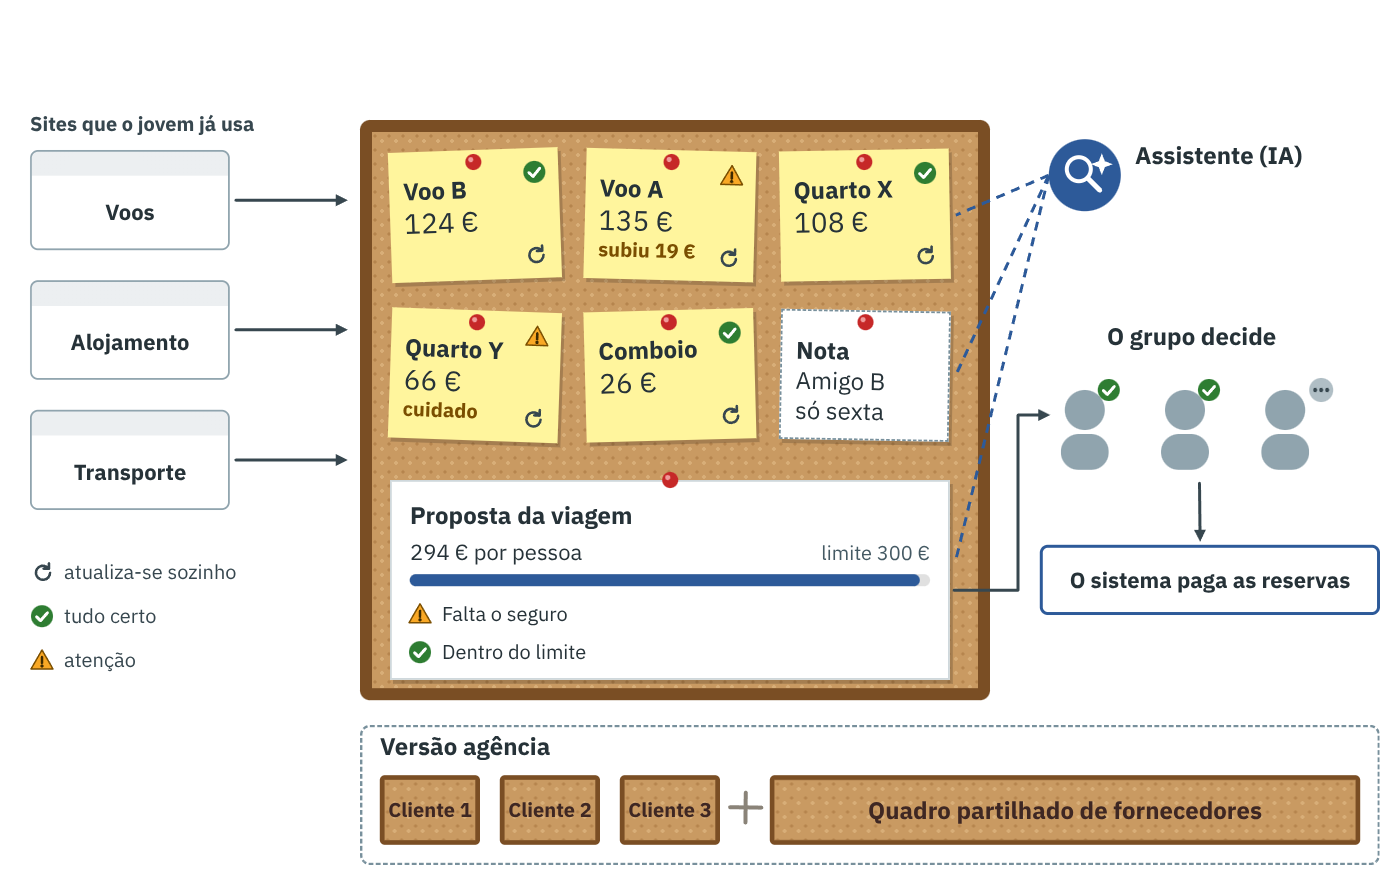
\includegraphics[width=\linewidth]{figuras/vision.png}
    \caption{Roamly: um quadro de cortiça que se atualiza sozinho}
\end{figure}
%==========================================================
\section{Interface de utilizador}\label{sec:interface}

Para a nossa interface, nós temos dois claros focos: o jovem cliente e o agente.
Nós supomos que o jovem cliente utiliza a versão base do nosso sistema Roamly, enquanto o agente utiliza a versão premium.
Para cada ponto de foco, temos 3 janelas que apresentam as funcionalidades principais do sistema.
Para fazer login, assumimos que uma janela para esse efeito aparecerá após a aplicação ser iniciada.
Para utilizadores com a versão base, login não é necessário.
Para fazer logout, basta clicar no nome do utilizador (que nas janelas do agente é "Agente C") para que um menu apareça, onde se possa fazer logout.

\subsection{Wireframes}

\begin{figure}[!ht]
  \centering
  % Pair 1
  \begin{subfigure}{0.45\textwidth}
    \centering
    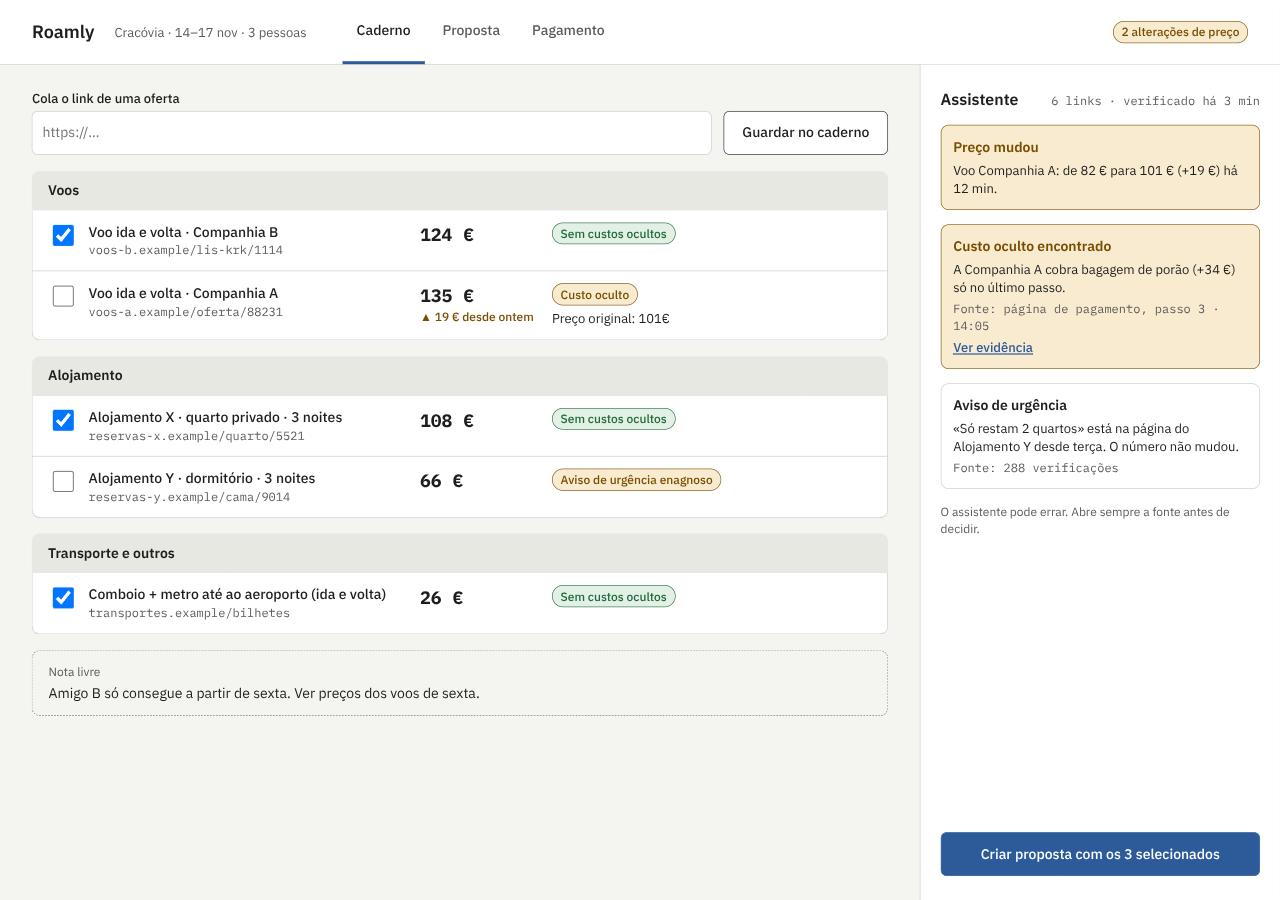
\includegraphics[width=\linewidth]{figuras/jovem1.png}
    \caption{Caderno de ofertas do Jovem}
  \end{subfigure}\hfill
  \begin{subfigure}{0.45\textwidth}
    \centering
    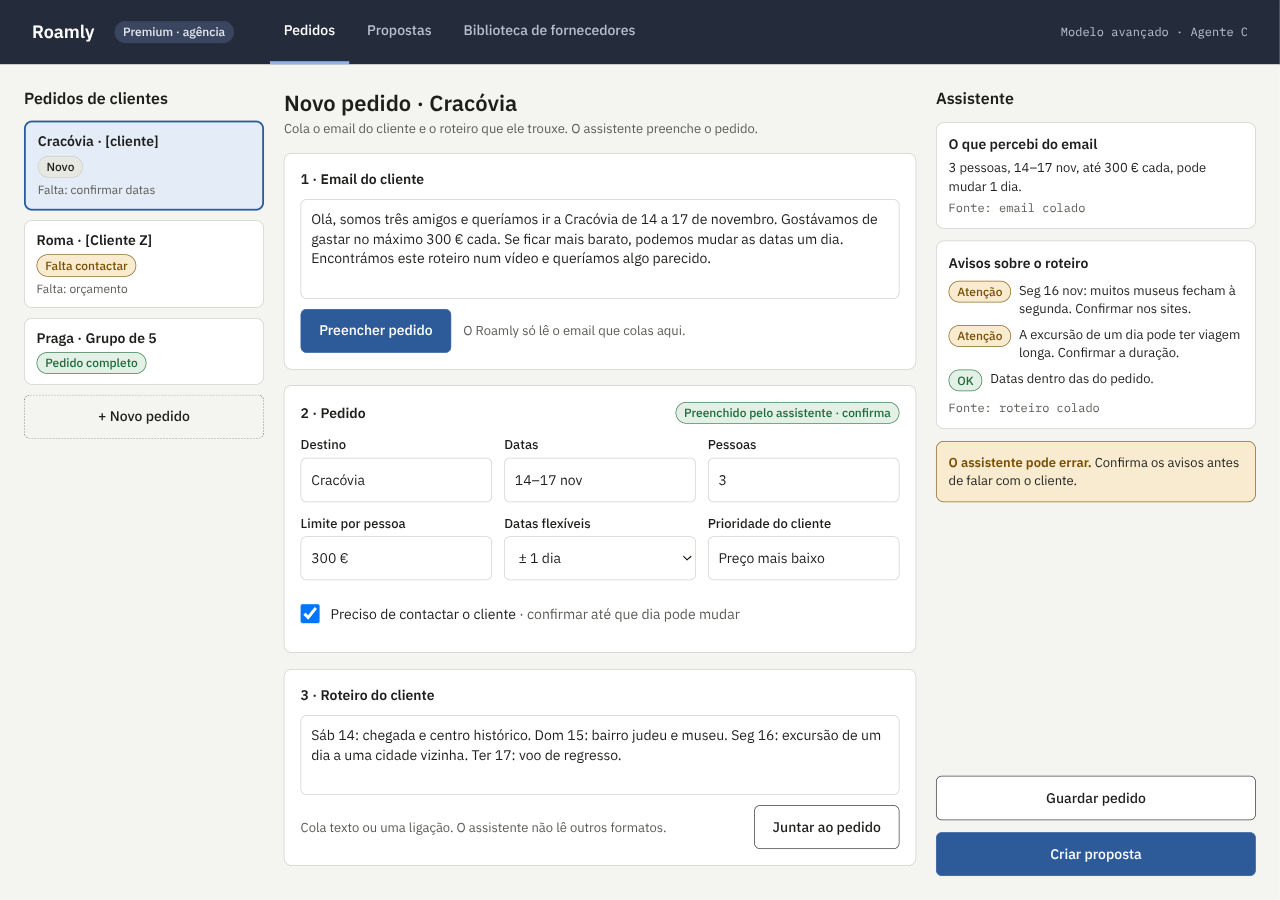
\includegraphics[width=\linewidth]{figuras/agente1.png}
    \caption{Pedidos dos clientes do Agente}
  \end{subfigure}\hfill
  \begin{subfigure}{0.45\textwidth}
    \centering
    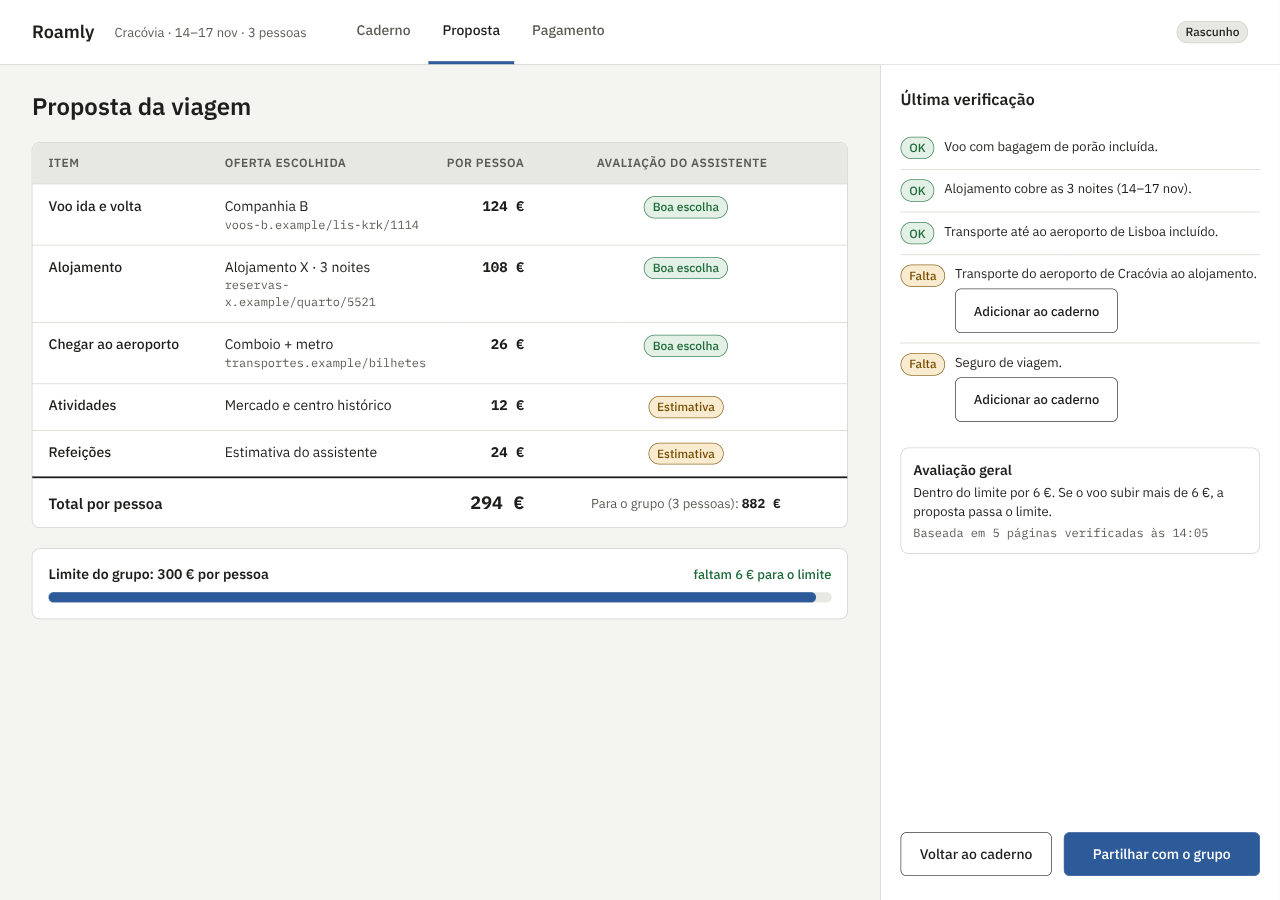
\includegraphics[width=\linewidth]{figuras/jovem2.png}
    \caption{Proposta de viagem do Jovem}
  \end{subfigure}\hfill
  \begin{subfigure}{0.45\textwidth}
    \centering
    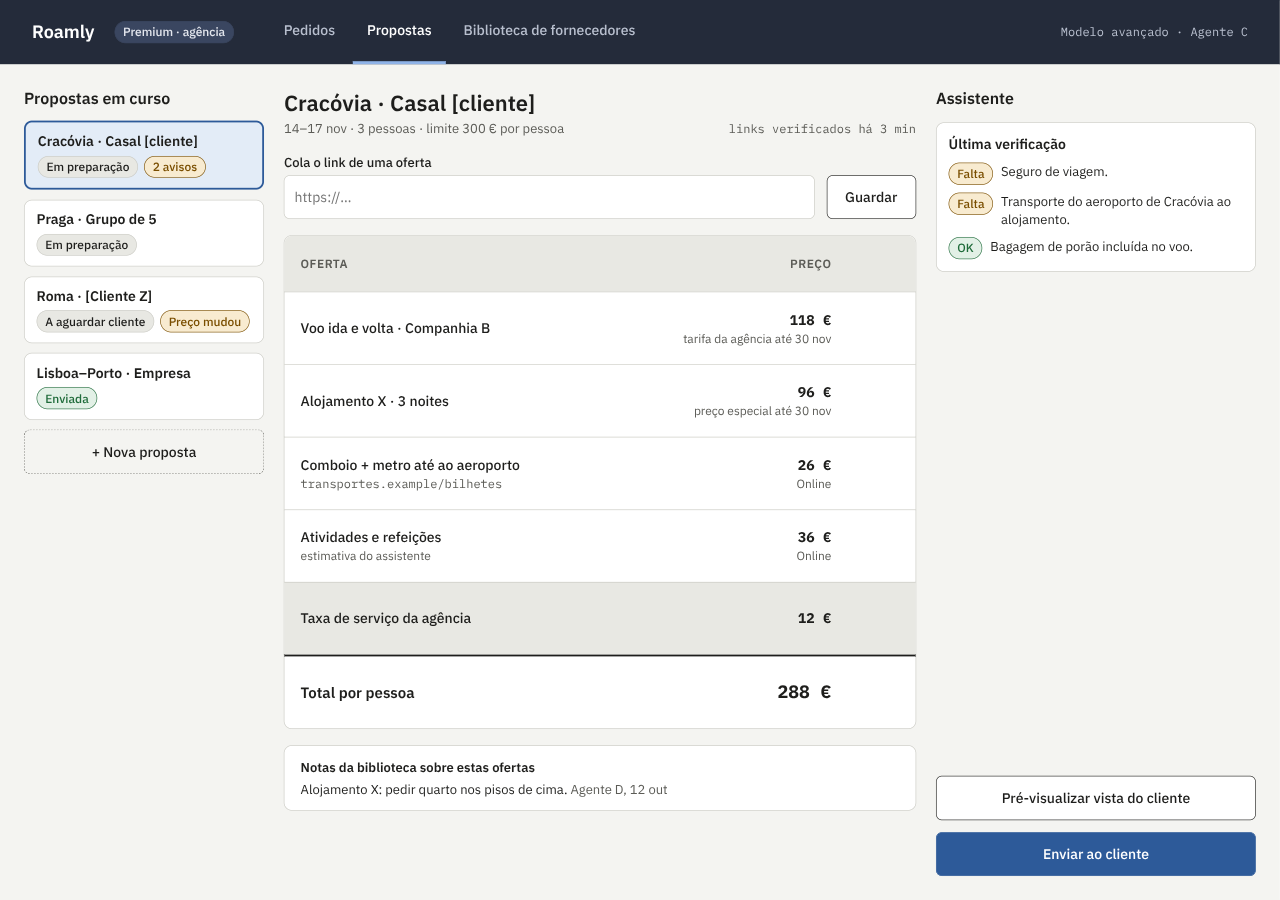
\includegraphics[width=\linewidth]{figuras/agente2.png}
    \caption{Proposta de viagem de um cliente do Agente}
  \end{subfigure}\hfill
  \begin{subfigure}{0.45\textwidth}
    \centering
    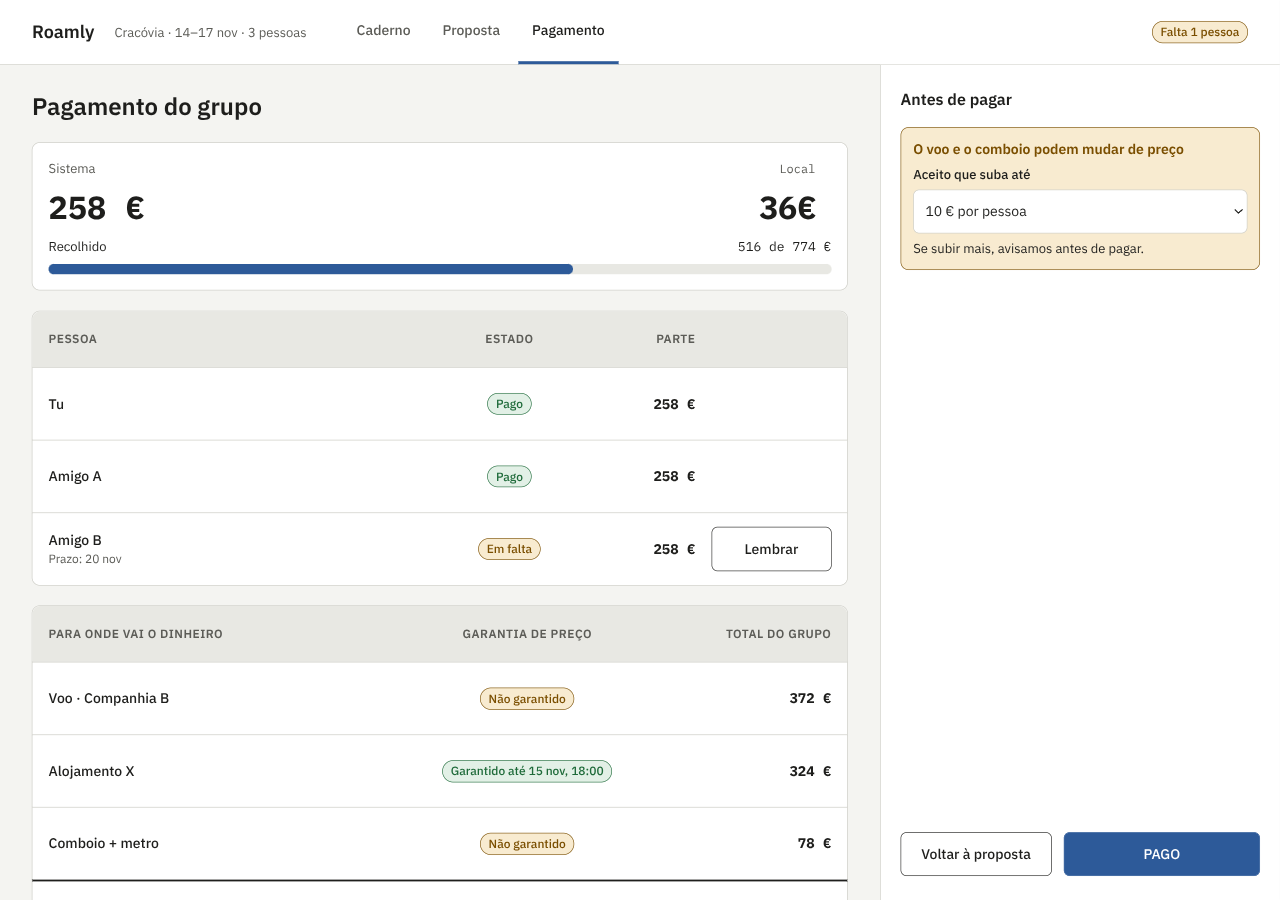
\includegraphics[width=\linewidth]{figuras/jovem3.png}
    \caption{Pagamento do Jovem e dos seus colegas}
  \end{subfigure}\hfill
  \begin{subfigure}{0.45\textwidth}
    \centering
    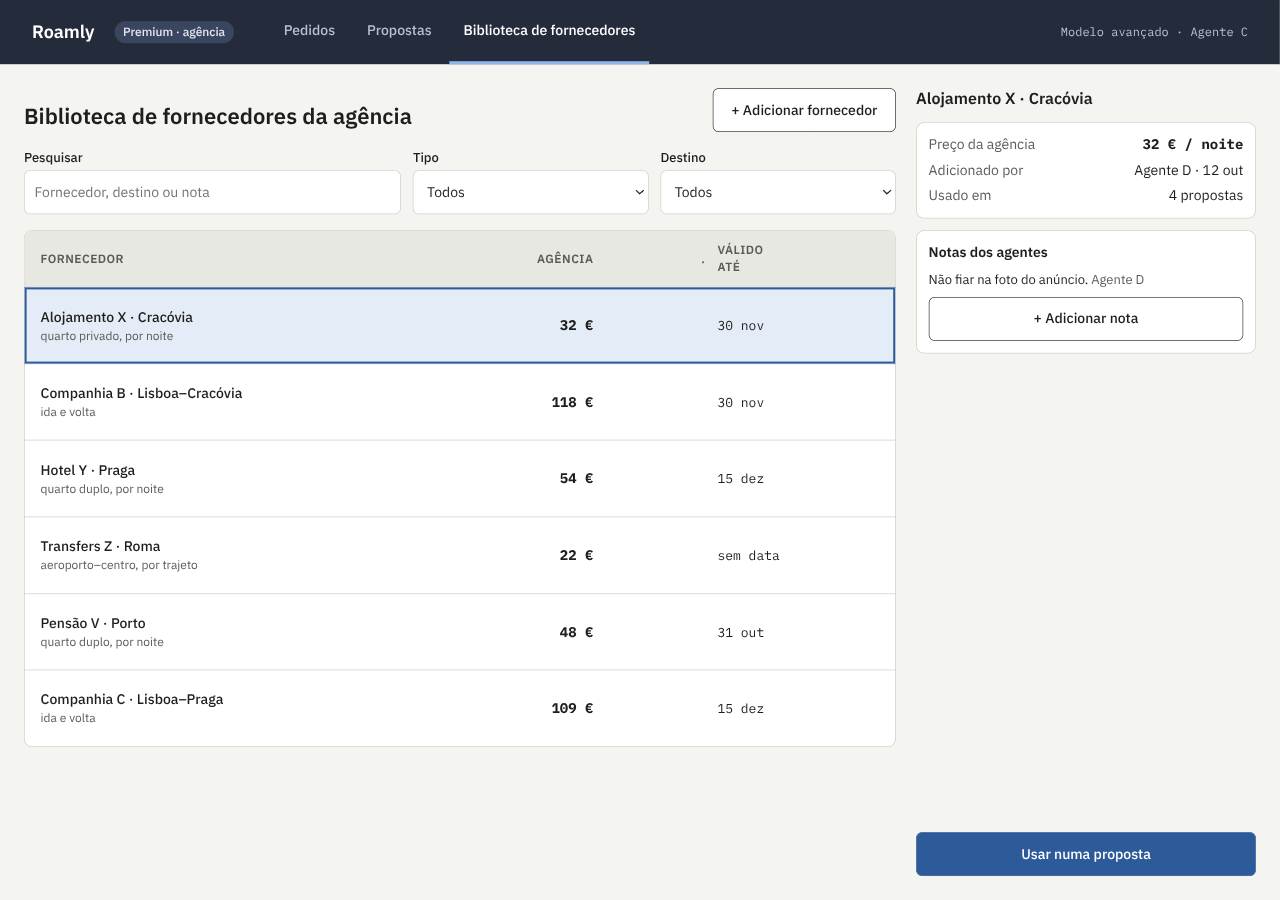
\includegraphics[width=\linewidth]{figuras/agente3.png}
    \caption{Biblioteca de fornecedores do Agente}
  \end{subfigure}\hfill
  \caption{6 janelas da nossa interface de utilizador. À esquerda, para o Jovem. À direite, para o Agente}
  \label{fig:three_pairs}
\end{figure}

\subsection{Avaliação de usabilidade de Nielsen}
%==========================================================
\section{Reflexão crítica}\label{sec:reflexao}

\pendente{Equipa}{%
Uma página, no máximo. O enunciado pergunta: \textbf{onde é que a avaliação heurística e o percurso cognitivo discordaram, e porquê?} Pontos a cobrir:
\begin{itemize}
  \item problemas que só uma das avaliações encontrou e porque é que a outra não os podia encontrar (as heurísticas olham para a interface como um todo; o percurso segue uma tarefa concreta de um utilizador concreto);
  \item problemas em que as duas discordaram na gravidade;
  \item o que isso diz sobre o protótipo e sobre os dados de campo em que assenta;
  \item o que a equipa faria de diferente na próxima iteração.
\end{itemize}}

%==========================================================
\section{Conclusões e próximos passos}\label{sec:conclusao}

\subsection{O que mudou na nossa compreensão do projeto}

Começámos com uma solução em mente: um agente de IA que junta voos, alojamento e atividades a partir do orçamento e das datas
e propõe um itinerário (Secção~\ref{sec:introducao}). As duas entrevistas mudaram a forma como vemos o problema em 2 pontos.

\begin{itemize}
  \item \textbf{Planear uma viagem de grupo é também coordenar pessoas e dinheiro.} O organizador é ao mesmo tempo planeador,
        coordenador e tesoureiro (Secção~\ref{sec:fluxo-cons}). Muitos \textit{breakdowns} não estão na pesquisa, mas na
        passagem para o grupo: respostas lentas, uma folha que ninguém abre e pagamentos em atraso (Tabela~\ref{tab:breakdowns}).
  \item \textbf{Para a agência, o valor está na preparação, não no aconselhamento.} O agente define-se por aconselhar e conhecer
        os fornecedores. O que lhe pesa é copiar dados entre sistemas e guardar num caderno pessoal o que «não está em lado
        nenhum». É aí que o \projeto{} o pode apoiar, sem o substituir.
\end{itemize}

\subsection{Limitações}

Estas conclusões assentam em duas entrevistas, um viajante e um agente, feitas pelo mesmo elemento da equipa e interpretadas
depois a partir do seu relato (Secção~\ref{sec:recolha}). Os padrões que encontrámos são indícios, não conclusões gerais.
Os amigos e a mãe de U0 só os conhecemos pelo que U0 contou, e não ouvimos viajantes que viajem sozinhos nem outros agentes.

\subsection{Questões em aberto}

\begin{itemize}
  \item Porque é que o grupo demora a responder: medo de se comprometer, falta de dinheiro ou desinteresse? 
  \item Quanto da receita da agência vem de comissões e quanto da taxa de serviço?
  \item Conseguimos obter preços completos, com os extras, sem violar os termos de uso dos fornecedores e das plataformas
        (Secção~\ref{sec:problema})?
\end{itemize}



%==========================================================
\begin{thebibliography}{9}

\bibitem{beyer1998}
H.~Beyer e K.~Holtzblatt.
\newblock \textit{Contextual Design: Defining Customer-Centered Systems}.
\newblock Morgan Kaufmann, San Francisco, 1998.

\bibitem{beyer1999}
H.~Beyer e K.~Holtzblatt.
\newblock Contextual design.
\newblock \textit{interactions}, 6(1):32--42, 1999.

\bibitem{holtzblatt1995}
K.~Holtzblatt e H.~Beyer (eds.).
\newblock Requirements gathering: the human factor.
\newblock \textit{Communications of the ACM}, 38(5), 1995.

\bibitem{nielsen1990}
J.~Nielsen e R.~Molich.
\newblock Heuristic evaluation of user interfaces.
\newblock Em \textit{Proceedings of ACM CHI'90}, pp.~249--256, 1990.

\bibitem{nielsen1994}
J.~Nielsen.
\newblock Enhancing the explanatory power of usability heuristics.
\newblock Em \textit{Proceedings of ACM CHI'94}, 1994.

\bibitem{wharton1994}
C.~Wharton, J.~Rieman, C.~Lewis e P.~Polson.
\newblock The cognitive walkthrough method: a practitioner's guide.
\newblock Em J.~Nielsen e R.~Mack (eds.), \textit{Usability Inspection Methods}, pp.~105--140. Wiley, 1994.

\end{thebibliography}


\clearpage
\begin{appendices}
%==========================================================
\section{Notas de campo}\label{anx:notas}

Este apêndice reproduz na íntegra os registos das duas sessões: perfil e situação da entrevista, conversa convencional, registos da entrevista contextual, fecho validado com o participante e notas da sessão de interpretação. São os documentos-fonte de todos os modelos deste relatório.

\begin{table}[!htbp]
\centering\small
\begin{tabularx}{\textwidth}{@{}p{3cm}Lp{2.6cm}@{}}
\toprule
\textbf{Sessão} & \textbf{Conteúdo} & \textbf{Página} \\
\midrule
A0: agente de viagens & Registos AE01--AE08 e notas A0-01--A0-15 & \pageref{anx:notas-a0} \\
U0: jovem viajante & Registos UE01--UE19 e notas U0-01--U0-21 & \pageref{anx:notas-u0} \\
\bottomrule
\end{tabularx}
\caption{Documentos de notas de campo incluídos neste apêndice.}
\label{tab:notas-campo}
\end{table}

\includepdf[pages=-,scale=0.88,frame,pagecommand={\thispagestyle{fancy}},
  addtotoc={1,subsection,2,{Sessão A0: agente de viagens de balcão},anx:notas-a0}]
  {\wm/interviews/agentes/A0-entrevista-agente.pdf}

\includepdf[pages=-,scale=0.88,frame,pagecommand={\thispagestyle{fancy}},
  addtotoc={1,subsection,2,{Sessão U0: jovem viajante},anx:notas-u0}]
  {\wm/interviews/viajantes/U0-entrevista-viajante.pdf}

%==========================================================
\section{Uso de IA generativa}\label{anx:ia}

O enunciado pede que, se a equipa usou um LLM para ajudar a agrupar notas de campo ou a redigir o guião do percurso cognitivo, mostre \textbf{um exemplo do que a IA errou}. Este anexo regista onde a IA foi usada, o que foi verificado à mão e o que teria ficado errado sem essa verificação.

\subsection{Onde foi usada}

\begin{table}[H]
\centering\small
\begin{tabularx}{\textwidth}{@{}p{3.4cm}LL@{}}
\toprule
\textbf{Tarefa} & \textbf{O que a IA fez} & \textbf{O que a equipa verificou ou mudou} \\
\midrule
Revisão dos registos de entrevista & Detetou incoerências entre registos, notas de interpretação e siglas (referências a registos inexistentes, siglas sem definição). & Cada correção foi aceite ou rejeitada pela equipa; a menção ao ChatGPT foi mantida contra a sugestão da IA. \\
Modelos culturais & Redesenhou os modelos com a notação do livro (direção das setas, voz do influenciador, \textit{pushback}, sobreposição). & Cada influência foi conferida com o registo que cita. \\
Consolidação do fluxo e do cultural & Propôs papéis, agrupamentos de influenciadores e nomes abstratos para comunicações e artefactos. & Papéis e agrupamentos revistos contra os modelos individuais. \\
Modelo do relatório & Gerou a estrutura em \LaTeX{} e o texto das secções já com dados. & \textit{a preencher} \\
Diagrama de afinidade & \textit{a preencher, se usada} & \\
Avaliação heurística e percurso cognitivo & \textit{a preencher, se usada} & \\
\bottomrule
\end{tabularx}
\caption{Uso de IA generativa nesta entrega.}
\label{tab:uso-ia}
\end{table}

\subsection{Exemplo do que a IA errou}

\pendente{Equipa}{%
Escolher o exemplo a apresentar e completá-lo (o que a IA produziu, porque estava errado, como foi detetado e como foi corrigido). Casos registados durante esta entrega:
\begin{itemize}
  \item \textbf{Sigla inventada.} O documento de A0 usava «F/OP» sem definir o «F». A IA propôs «fala geral» e escreveu essa definição no glossário, sem base nos dados. A definição tem de ser confirmada ou corrigida pela equipa.
  \item \textbf{Classificação de registos} (só serve se essa versão tiver sido gerada com IA; confirmar). Na versão inicial de U0, acontecimentos passados noutros locais (por exemplo, «no corredor, entre aulas») estavam marcados como O (observado), embora o entrevistador não pudesse tê-los visto. Passaram a R (relato).
  \item \textbf{Contagem errada.} Ao resumir as sessões, a IA indicou 7 registos observados e 12 relatos em U0; a contagem correta é 8 e 11.
  \item \textbf{Pressuposto sobre a equipa.} Ao distribuir os papéis das sessões de interpretação, a IA assumiu quem tinha entrevistado A0 e U0 sem que isso estivesse nos dados.
\end{itemize}
Se a IA for usada no diagrama de afinidade, a comparação entre os agrupamentos da IA e os da equipa (padrões inventados, perda da origem das notas) é o exemplo mais relevante para o enunciado.}

%==========================================================
\section{Organização da equipa}\label{anx:organizacao}

Cada tipo de modelo tem um dono, que define a notação final e revê todos os modelos desse tipo, e um suplente, para que o conhecimento não dependa de uma só pessoa.

\begin{table}[H]
\centering\small
\begin{tabularx}{\textwidth}{@{}p{3.6cm}Lp{2.2cm}p{2.2cm}@{}}
\toprule
\textbf{Responsabilidade} & \textbf{Âmbito} & \textbf{Dono} & \textbf{Suplente} \\
\midrule
Fluxo & Notação, exemplo e revisão de todos os fluxos & Tiago & Gonçalo \\
Cultural & Idem, e das «vozes» das setas & Tiago & Gonçalo \\
Sequência & Idem, e das intenções e gatilhos & Gonçalo & Zé Pedro \\
Artefacto & Idem, e do arquivo anonimizado de artefactos & Gonçalo & Zé Pedro \\
Físico & Idem & Zé Pedro & Tiago \\
Guardião do processo & Calendário, rotação de papéis, consentimentos, repositório & Zé Pedro & Tiago \\
\bottomrule
\end{tabularx}
\caption{Donos e suplentes de cada modelo.}
\label{tab:donos}
\end{table}

Nas sessões de interpretação os papéis rodam, para que todos desenhem todos os tipos de modelo e ninguém modele sozinho a sua própria entrevista. Só o modelo físico é desenhado pelo entrevistador.

\begin{table}[H]
\centering\small
\begin{tabularx}{\textwidth}{@{}p{3.6cm}Lp{2.2cm}p{2.2cm}@{}}
\toprule
\textbf{Papel na sessão} & \textbf{Desenha} & \textbf{A0} & \textbf{U0} \\
\midrule
Entrevistador(a) & Físico; conta a entrevista pela ordem & Tiago & Gonçalo \\
Modelador(a) A & Fluxo e cultural; acrescenta notas & Gonçalo & Zé Pedro \\
Modelador(a) B & Sequência e artefacto & Zé Pedro & Tiago \\
\bottomrule
\end{tabularx}
\caption{Rotação de papéis nas sessões de interpretação.}
\label{tab:rotacao}
\end{table}

\pendente{Equipa}{Confirmar quem entrevistou A0 e U0 e ajustar a Tabela~\ref{tab:rotacao}. Acrescentar a contribuição de cada elemento para esta entrega (o enunciado prevê um inquérito de contribuição dentro da equipa).}

\end{appendices}

\end{document}
